\documentclass[xcolor={usenames,dvipsnames,svgnames}, compress]{beamer}

% \usepackage[utf8]{inputenc}
\usepackage{booktabs}
\usepackage{dcolumn}
\usepackage{colortbl}

% \usepackage[style=authoryear-comp, backref=true]{biblatex}
\usepackage{ifxetex}
\usepackage{amsmath}
\usepackage{biblatex}
% 
\usepackage[no-math]{fontspec}

\usetheme{enziteto}
% 
% CLIPS listings
%\usepackage[utf8]{inputenc}
\usepackage{listings}
\usepackage{xcolor}


%
% I asked on stackoverflow for rainbow parentheses
% http://tex.stackexchange.com/questions/235740/rainbow-parentheses-in-lisp-listings
% the palette is from solarized theme
\definecolor{solarized-cyan}{RGB}{42, 161, 152}
\definecolor{solarized-magenta}{RGB}{211, 54, 130}
\definecolor{solarized-yellow}{RGB}{181, 137, 0}
\definecolor{solarized-violet}{RGB}{108, 113, 196}
\definecolor{solarized-red}{RGB}{220, 50, 47}
\definecolor{solarized-orange}{RGB}{203, 75, 22}
\definecolor{solarized-grey}{RGB}{101, 123, 131}

\lstdefinelanguage{clips}
{
  classoffset=0,
  morekeywords ={deffunction, deftemplate, defglobal, defmodule, defrule, deffacts, nil, assert, retract},
  keywordstyle=\bfseries\color{solarized-orange},
  classoffset=1,
  morekeywords ={delcare, salience, run, slot, multislot, clear, reset, facts, exit, agenda, initial-fact, watch, ppdefrule, unwatch, printout, if, then, else, while, loop-count, crlf, read, readline},
  keywordstyle=\bfseries,
  %classoffset=2,
  %keywordsprefix=\?,
  %alsoletter=\?,
  %keywordstyle=\itshape\color{solarized-red},
  classoffset=0,
  sensitive=true,
  morecomment=[l]{;},
  morestring=[b]{"},
  stringstyle=\color{solarized-grey},
  basicstyle=\scriptsize,%\ttfamily\scriptsize,
  numbers=left,
  numbersep=-5pt,
  numberstyle=\tiny,
  showstringspaces=false,
  }

\renewcommand{\ttdefault}{pcr}

% egreg's modulo macro (see http://tex.stackexchange.com/a/34449/21891)
\def\truncdiv#1#2{((#1-(#2-1)/2)/#2)}
\def\moduloop#1#2{(#1-\truncdiv{#1}{#2}*#2)}
\def\modulo#1#2{\number\numexpr\moduloop{#1}{#2}\relax}    

\makeatletter

% a TeX counter to keep track of the nesting level
\newcount\netParensCount@clisp

% Modify how ( and ) get typeset depending on the value of the counter
% (Based on Ulrike Fischer's approach to modifying characters in listings;
% see http://tex.stackexchange.com/a/231927/21891)
\lst@CCPutMacro
\lst@ProcessOther{`(}{{%
    \ifnum\lst@mode=\lst@Pmode\relax%
    \rainbow@clisp{(}%
    \global\advance\netParensCount@clisp by \@ne%
    \else
    (%
    \fi
  }}%
\lst@ProcessOther{`)}{{%
    \ifnum\lst@mode=\lst@Pmode\relax%
    \global\advance\netParensCount@clisp by \m@ne%
    \rainbow@clisp{)}%
    \else
    )%
    \fi
  }}%
\@empty\z@\@empty
% Color its argument based on the value of the \netParensCount@clisp counter
% (modulo 5)
\newcommand\rainbow@clisp[1]{%
  \ifcase\modulo\netParensCount@clisp 5\relax%
  \textcolor{solarized-cyan}{\bfseries#1}%
  \or
  \textcolor{solarized-yellow}{\bfseries#1}%
  \or
  \textcolor{solarized-magenta}{\bfseries#1}%
  \or
  \textcolor{solarized-violet}{\bfseries#1}%
  \else
  \textcolor{solarized-red}{\bfseries#1}%
  \fi
}

% Alternatively, you could simplify the definition of \rainbow@clisp to...
% \newcommand\rainbow@clisp[1]{%
% \textcolor{color\modulo\netParensCount@clisp 5}{#1}%
% }
%   ... but this assumes that the colours have names of the form color<i>,
%   where <i> is a positive integer

%   reset the counter at the beginning of each listing
%   (just in case there were unmatched parentheses in a previous listing)
\lst@AddToHook{PreInit}{%
  \global\netParensCount@clisp 0\relax%
}

\makeatother




\lstnewenvironment{clips-code}[1][]
{\lstset{language=clips,
    #1
  }}
{}






%%% Local Variables:
%%% mode: latex
%%% TeX-master: t
%%% End:


\definecolor{jess-fucsia}{RGB}{170, 0, 127}
\definecolor{violent-green}{RGB}{0, 128, 96}
\definecolor{ny-orange}{RGB}{255, 128, 0}

\hypersetup{
  colorlinks=true,       % false: boxed links; true: colored links
  linkcolor=jess-fucsia,          % color of internal links (change box color with linkbordercolor)
  % citecolor=green,        % color of links to bibliography
  %filecolor=magenta,      % color of file links
  urlcolor=jess-fucsia           % color of external links
}

%%% Local Variables:
%%% mode: latex
%%% TeX-master: t
%%% End:


\setbeamertemplate{headline}{}

%%%%%%%%%%%%%%%%%%%%%%%%%%%%%%%%%%%%%%%%%%%%%%%%%%%%%%%%%%%% 
%%%%%%%%%%%%%%%%%%%%%%%%%%%%%%%%%%%%%%%%%%%%%%%%%%%%%%%%%%%% 
%%%%%%%%%%%%%%%%%%%%%%%%%%%%%%%%%%%%%%%%%%%%%%%%%%%%%%%%%%%% 


\begin{document}

\title{CLIPS: Knowledge Representation and Problem Solving}
%\subtitle{An Introduction}
\author{Antonio Vergari}
% \institute{Lacam$@$DIB$@$Uniba}
\institute{Università degli Studi di Bari}
\department{Dipartimento di Informatica}
\laboratory{LACAM}
\group{Machine Learning}
\institutelogo{
\includegraphics[width=25pt]{Figures/unibaba}}
\lablogo{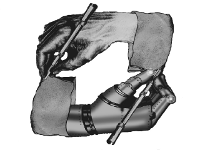
\includegraphics[width=35pt]{Figures/lacam}}

\footnotesize \let\small\footnotesize





{
  \setbeamertemplate{headline}{}
  \setbeamertemplate{footline}{}
  \begin{frame}
    \titlepage
  \end{frame}
}

\section{Knowledge Representation}
{\setbeamertemplate{headline}{}
  \begin{frame}
    \sectionpage
  \end{frame}
}

\begin{frame}
  \frametitle{A simple diagnostic classifier}
  Getting back to the previous example, the knowledge we wanted to
  embed could be expressed in such a few rules:
  \begin{enumerate}[I.]
  \item \textbf{If} the skin and eyes are yellowish, \textbf{then}
    there is \emph{icterus} (partial diagnosis)
  \item  \textbf{If} the eyes are yellowish but not the skin, \textbf{then} there is
    \emph{scleral icterus} (partial diagnosis)
  \item \textbf{If} scleral icterus is present, there is no fever, and the
    patient's stressed or without food, \textbf{then} \emph{Gilbert's syndrome} can be
    diagnosed
  \item  \textbf{If} icterus is present, there is fever, the patient is young
    and tired, dyspepsia has been diagnosed and the liver is enlarged,
    \textbf{then} \emph{Acute viral hepatitis} can be diagnosed
  \item  \textbf{If} there is icterus, fever and the patient is not young but
    has recurrent pains and cholecyst pains, \textbf{then} it is  \emph{cholecystitis}
  \item \textbf{If} there is icterus, there is no fever and the patient is not
    young and abuses alchool, the liver is enlarged and the spleen is
    enlarged as well, \textbf{then} it is \emph{alchoolic cirrhosis}
  \end{enumerate}

\end{frame}

\begin{frame}[fragile]
  \frametitle{A very simple conceptualization}
  The minimal information needed to represent a symptom as a fact is
  its name and its presence. In this way we are limiting possible
  extensions (like user profiling), plus each precondition is treated
  as a symptom.
  \begin{clips-code}[numbers=none]
    (deftemplate symptom
        (slot name (type SYMBOL))
        (slot observed (default FALSE)))
  \end{clips-code}

  Thus a diagnostic rule could take this linear form:
  \begin{clips-code}[numbers=none]
    (defrule alchoolic-cirrhosis
        (symptom (name icterus) (observed TRUE))
        (symptom (name fever) (observed FALSE))
        (symptom (name young) (observed FALSE))
        (symptom (name alcohol-abuse) (observed TRUE))
        (symptom (name enlarged-liver) (observed TRUE))
        (symptom (name enlarged-spleen) (observed TRUE))
        =>
        (assert (diagnosis "Alchoolic cirrhosis")))
  \end{clips-code}
  
  In the case of partial diagnosis we will assert symptom facts and
  not diagnosis (this is a limitation as well).
\end{frame}

\begin{frame}[fragile,t]
  \frametitle{A more complex conceptualization}
  In the previous example we are assuming our expert system user to
  deal with a patient at a time. At each run, only \emph{his} symptoms
  are stored as facts in memory.\par
  However, suppose that your expert system shall do inference on
  \emph{different} patients' symptoms. In this case, it would be
  necessary to represent each patient as a fact, maybe with a
  template:
  \begin{clips-code}[numbers=none]
    (deftemplate patient
        (slot patient-name (type SYMBOL))
        (multislot symptoms (type SYMBOL)))
 \end{clips-code}

 Now, consider the problem of representing one patient symptom history
 instead. We would need a way to trace the previous diagnosis and
 their dates:

 \begin{clips-code}[numbers=none]
   (deftemplate symptom-diagnosis
       (slot name (type SYMBOL))
       (slot date (type STRING)))
 \end{clips-code} 
 
 in the end, the fact representation chosen highly depends on the
 conceptualization followed and the \emph{requirements} analysed\dots
\end{frame}

\begin{frame}[t]
  \frametitle{Modeling domains, experts, users}
  \framesubtitle{Some advices}
  Designing an expert system means to express an expert knowledge in
  terms of rules (and facts). Before designing it, be sure to well define all
  the requirements.\par\bigskip

  First determine a domain. Stick to some field you know. And for
  which encoding an expert knowledge in a software can be meaningful.\par\bigskip
  Then select which expert figure you are going to extract knowledge
  from. Find . You can be your own expert as well. 
  \par\bigskip
  Then model the system user. Is he an expert? a novice? When shall
  he consult the expert system? Keep in mind \emph{interactivity}.\par\bigskip

  You could use the requirements analysis techniques you studied up to
  now: interviews, questionnaires,\dots\par
  Properly write them down (a documentation is required), and \emph{simulate} a user-expert system interaction.
  
\end{frame}

\begin{frame}
  \frametitle{Rule Hierarchy I}
  To exend the first simple formalism one can conceptualize what some
  symptoms really mean and how to observe them in more depth.
  This can be done from the rule point of view as well.\par\bigskip

  For instance, what does it mean for a  patient to be young? Or to
  have the fever? We can add additional rules acting as \emph{mini-classifiers}.\par\bigskip
  {\color{ny-orange}\textbf{If} the patient's age is less than 25 years, \textbf{then} he's young, \textbf{otherwise if}
  it is still less than 50, \textbf{then} it is an adult, \textbf{else} an
  elder.\par
  \textbf{If} the patient's temperature is higher than 37.1 Celsius degrees,
  \textbf{then} he has a fever.\par \bigskip}

  We are clearly defining different stages in the diagnosis process,
  refining available information and collecting missing
  information. At the same time the interaction (via questions) shall
  be more focused and complex.\par
  One has to carefully design the set of rules forming his KB.
  
   
\end{frame}

\begin{frame}
  \frametitle{Rule Hierarchy II}
  To help you design a complex and consistent rule KB, writing them
  down is a good starting point.\par
  A rule can be thought of a joint, linking some facts (matching its
  LHS) to some newly asserted facts (from its RHS).\par
  Multiple rules can share some LHS patterns as well as some RHS
  slots. Connecting all the rules on paper in a \emph{rule graph} gives a hint of the system
  inner workings.
  \begin{center}
    \begin{minipage}{0.33\linewidth}
      \centering
      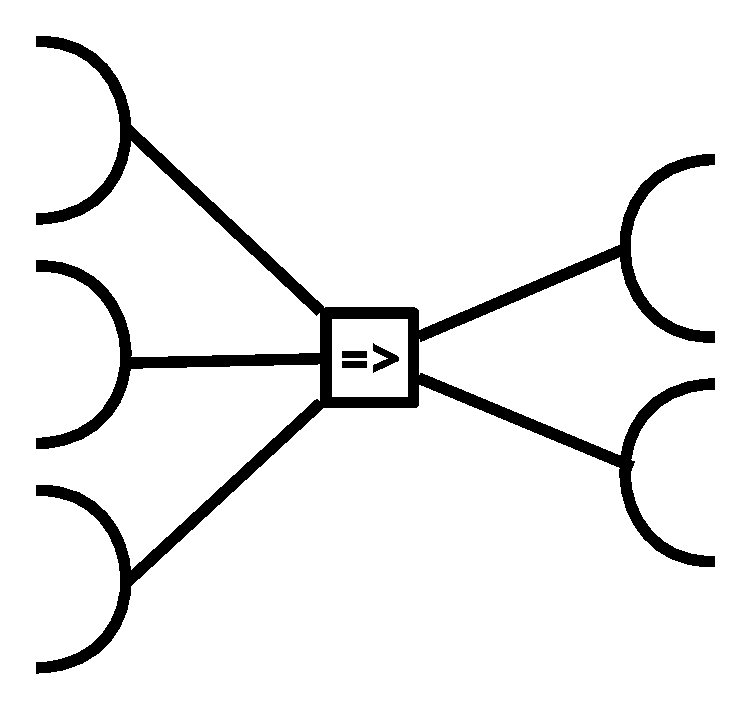
\includegraphics[width=0.7\linewidth]{Figures/rules-I}
    \end{minipage}\begin{minipage}{0.33\linewidth}
      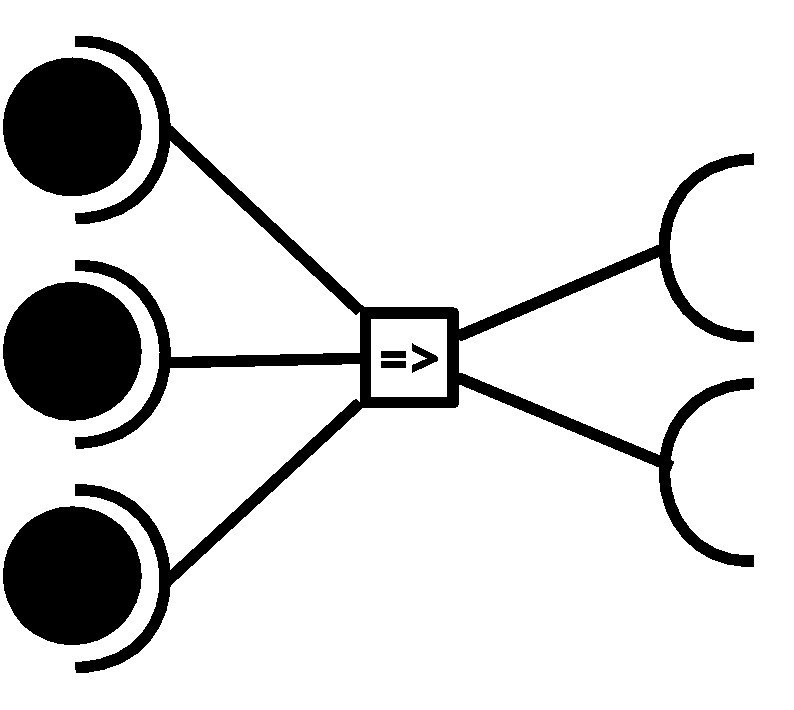
\includegraphics[width=0.7\linewidth]{Figures/rules-II}
    \end{minipage}\begin{minipage}{0.33\linewidth}
      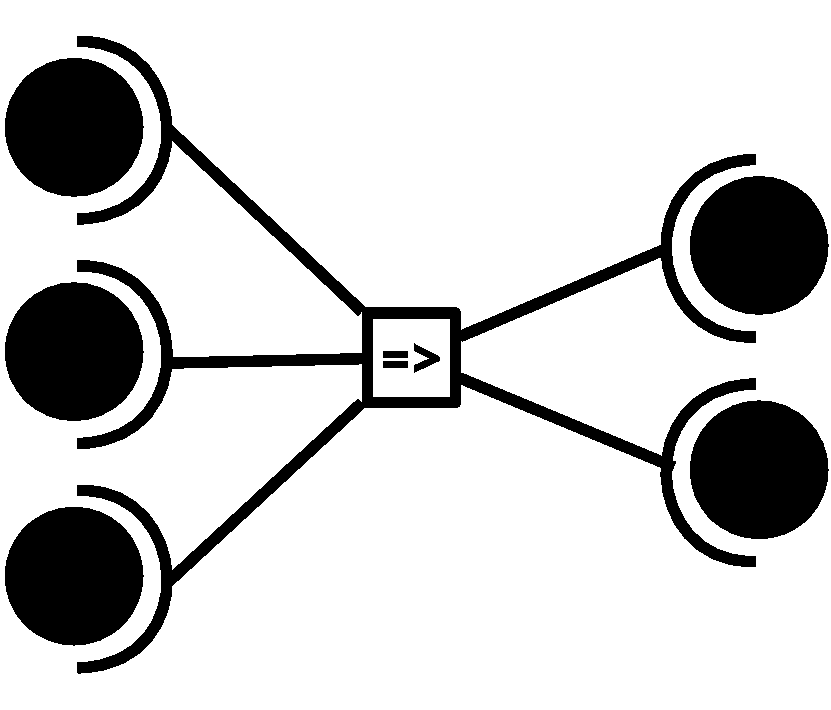
\includegraphics[width=0.7\linewidth]{Figures/rules-III}
    \end{minipage}
  \end{center}

  A \emph{non-linear} expert system shall activate different rules to
  different assertions. That is, different paths in the graphs are
  activated (maybe starting from the same point).
\end{frame}

\begin{frame}
  \frametitle{Rule Hierarchy III}
  Imagine a rule hierarchy written as a graph with three distinct
  possible outputs (classification results).
  \begin{center}
    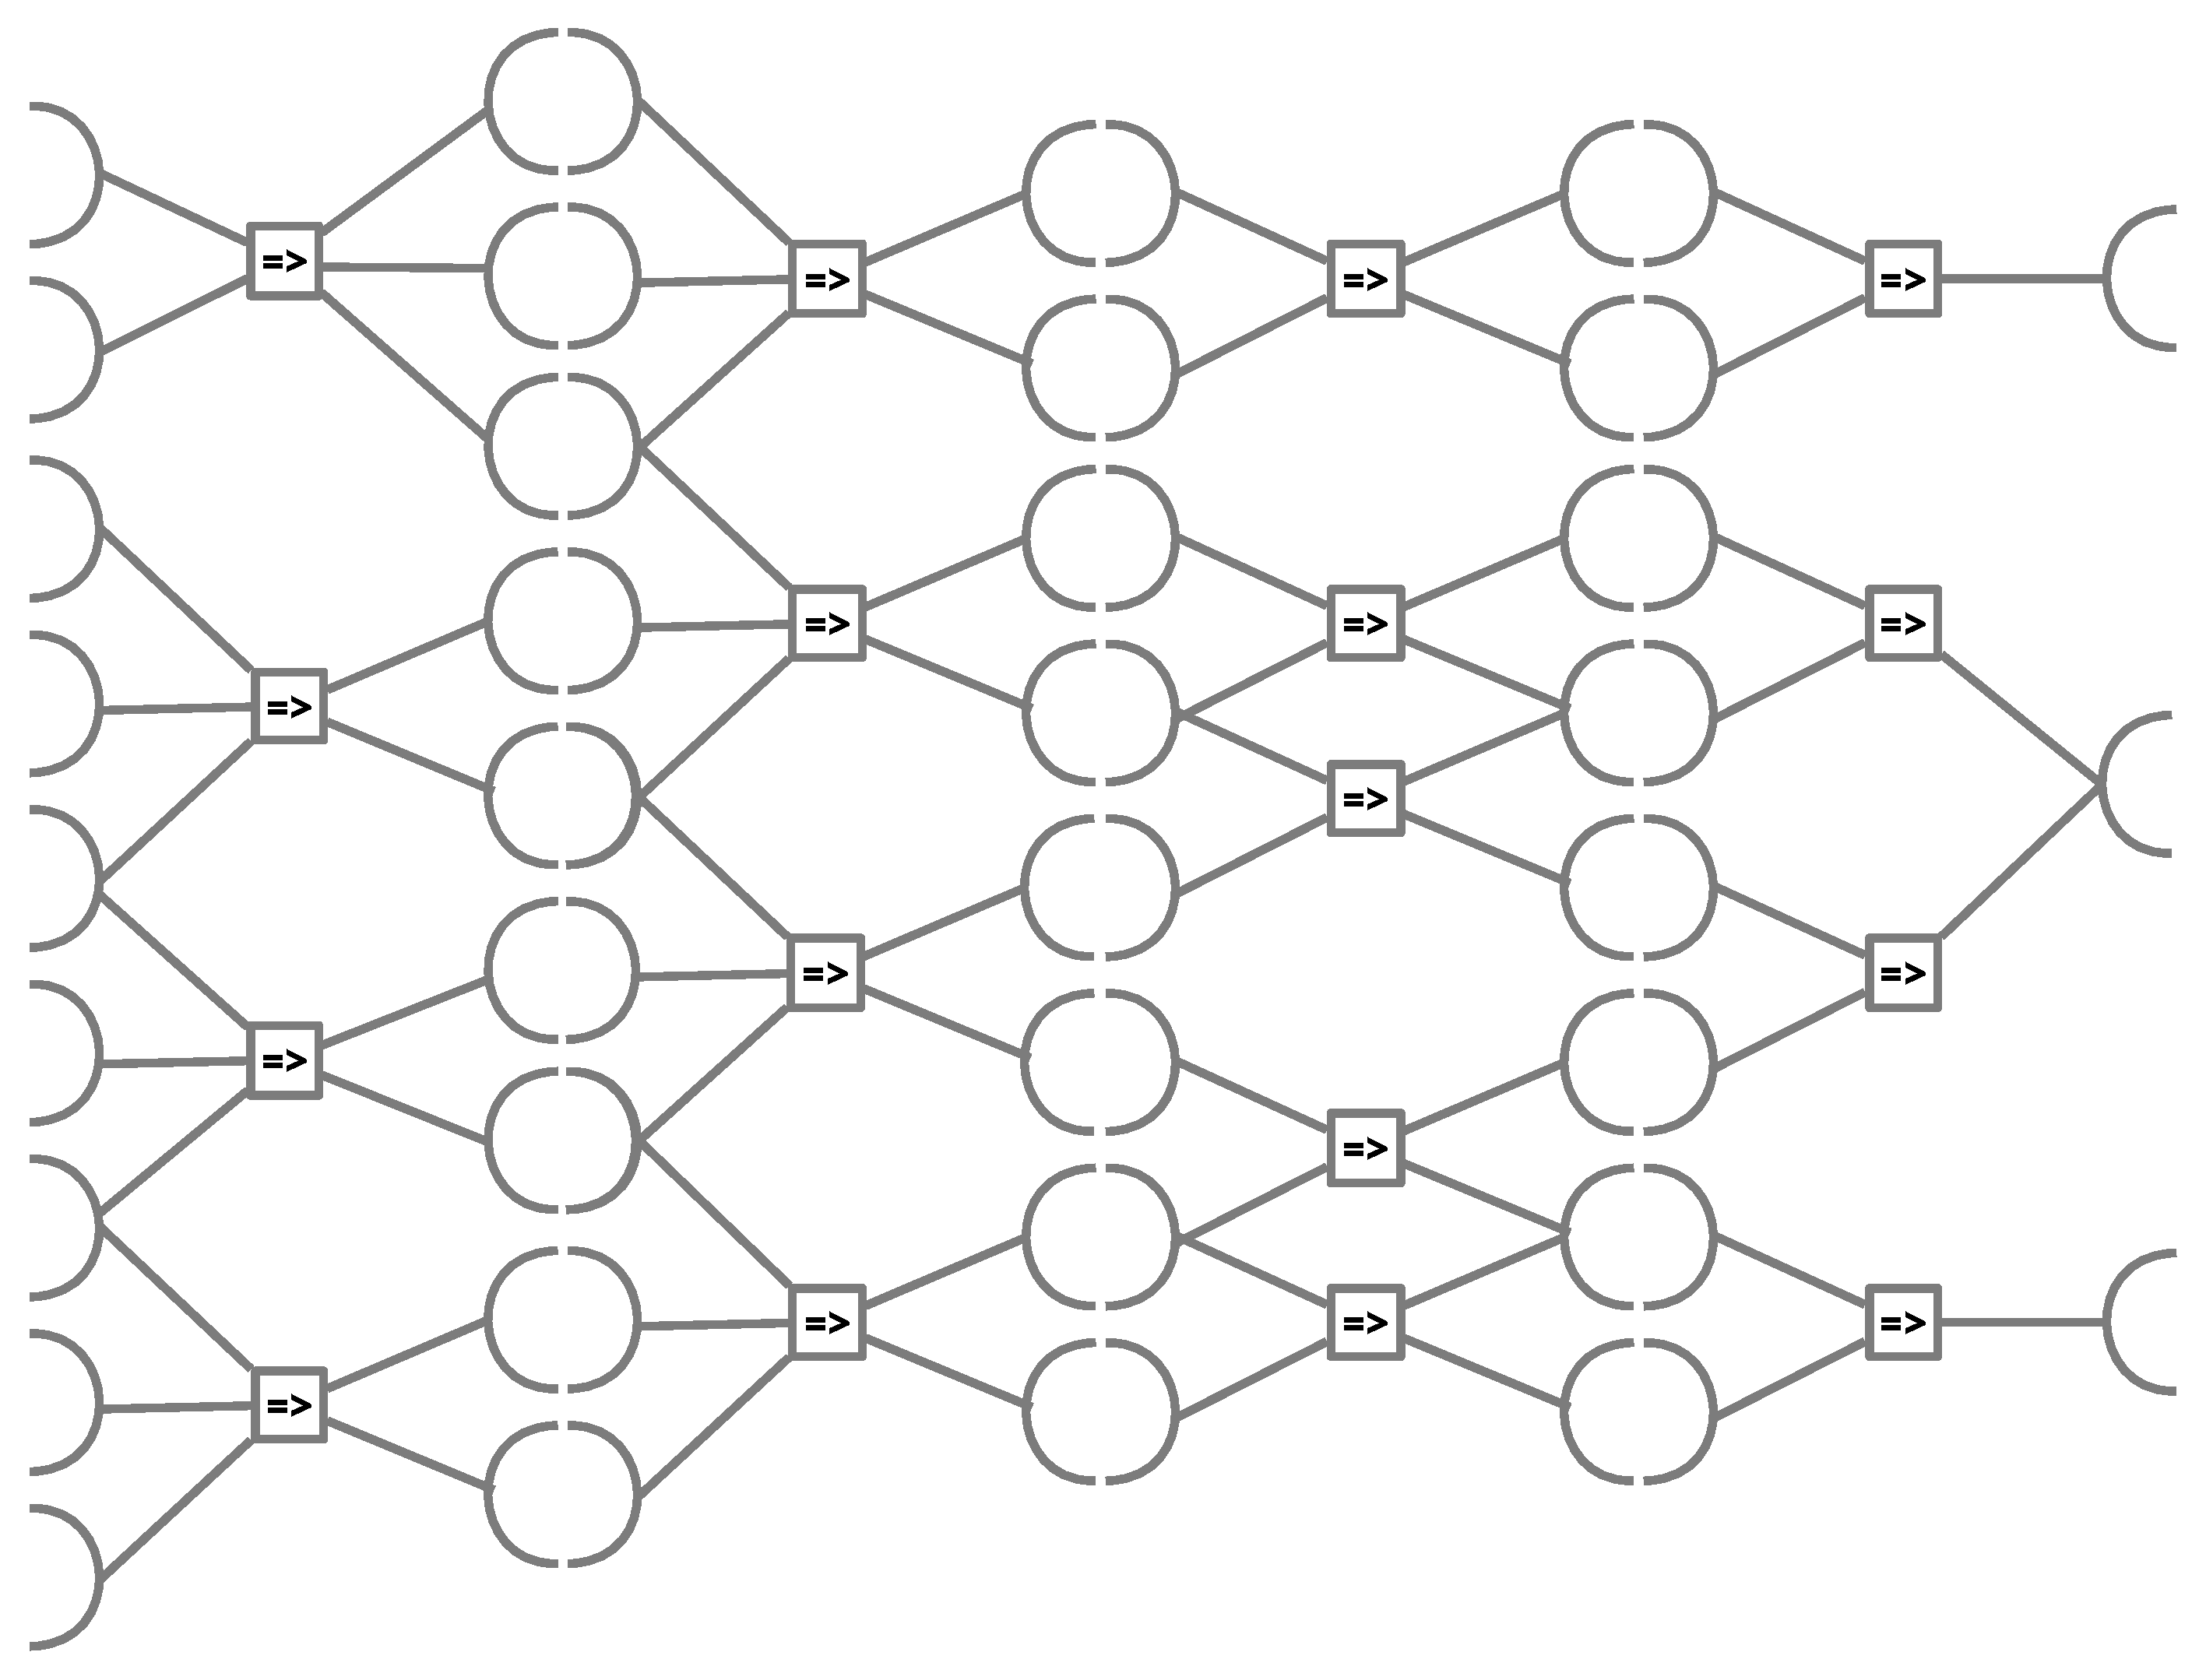
\includegraphics[width=0.7\linewidth]{Figures/rulesact}
  \end{center}
\end{frame}

\begin{frame}
  \frametitle{Rule Hierarchy IV}
  The facts asserted at the beginning determine the \emph{root} of the
  activation path.
  \begin{center}
    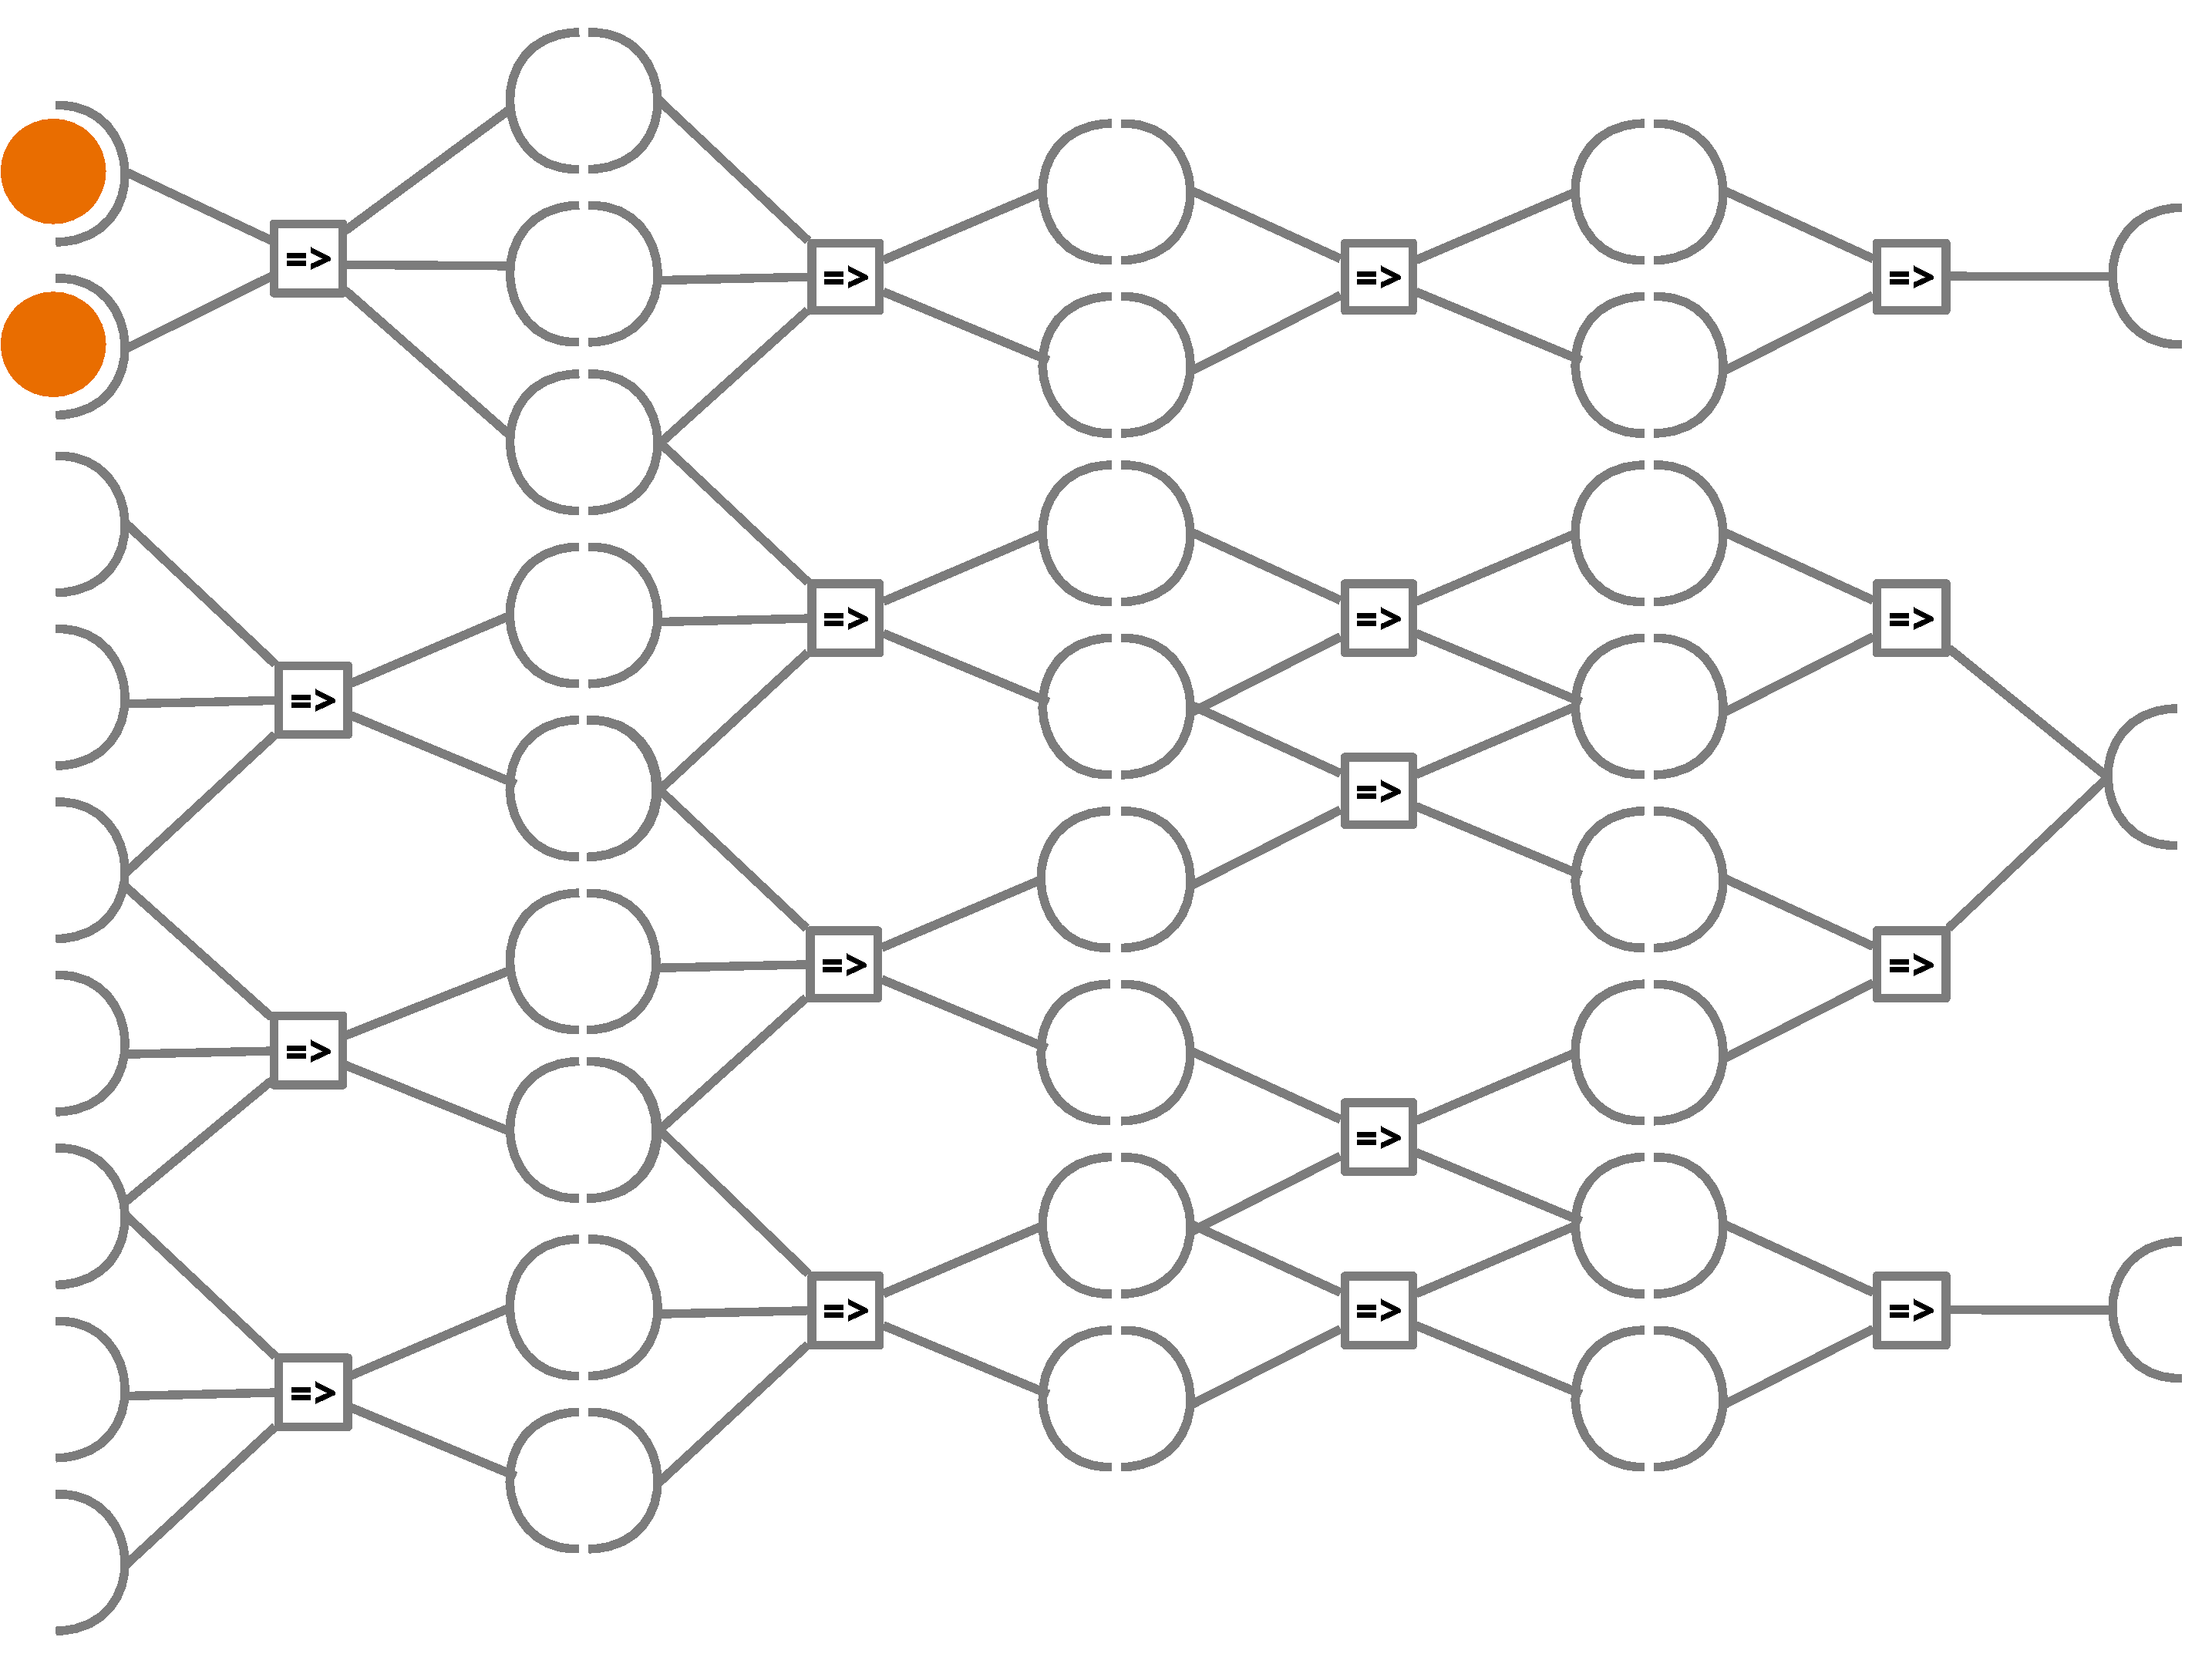
\includegraphics[width=0.7\linewidth]{Figures/rulesact-I}
  \end{center}
\end{frame}

\begin{frame}
  \frametitle{Rule Hierarchy V}
  When a LHS side of a rule gets satisfied we traverse it (we color
  it). 
  \begin{center}
    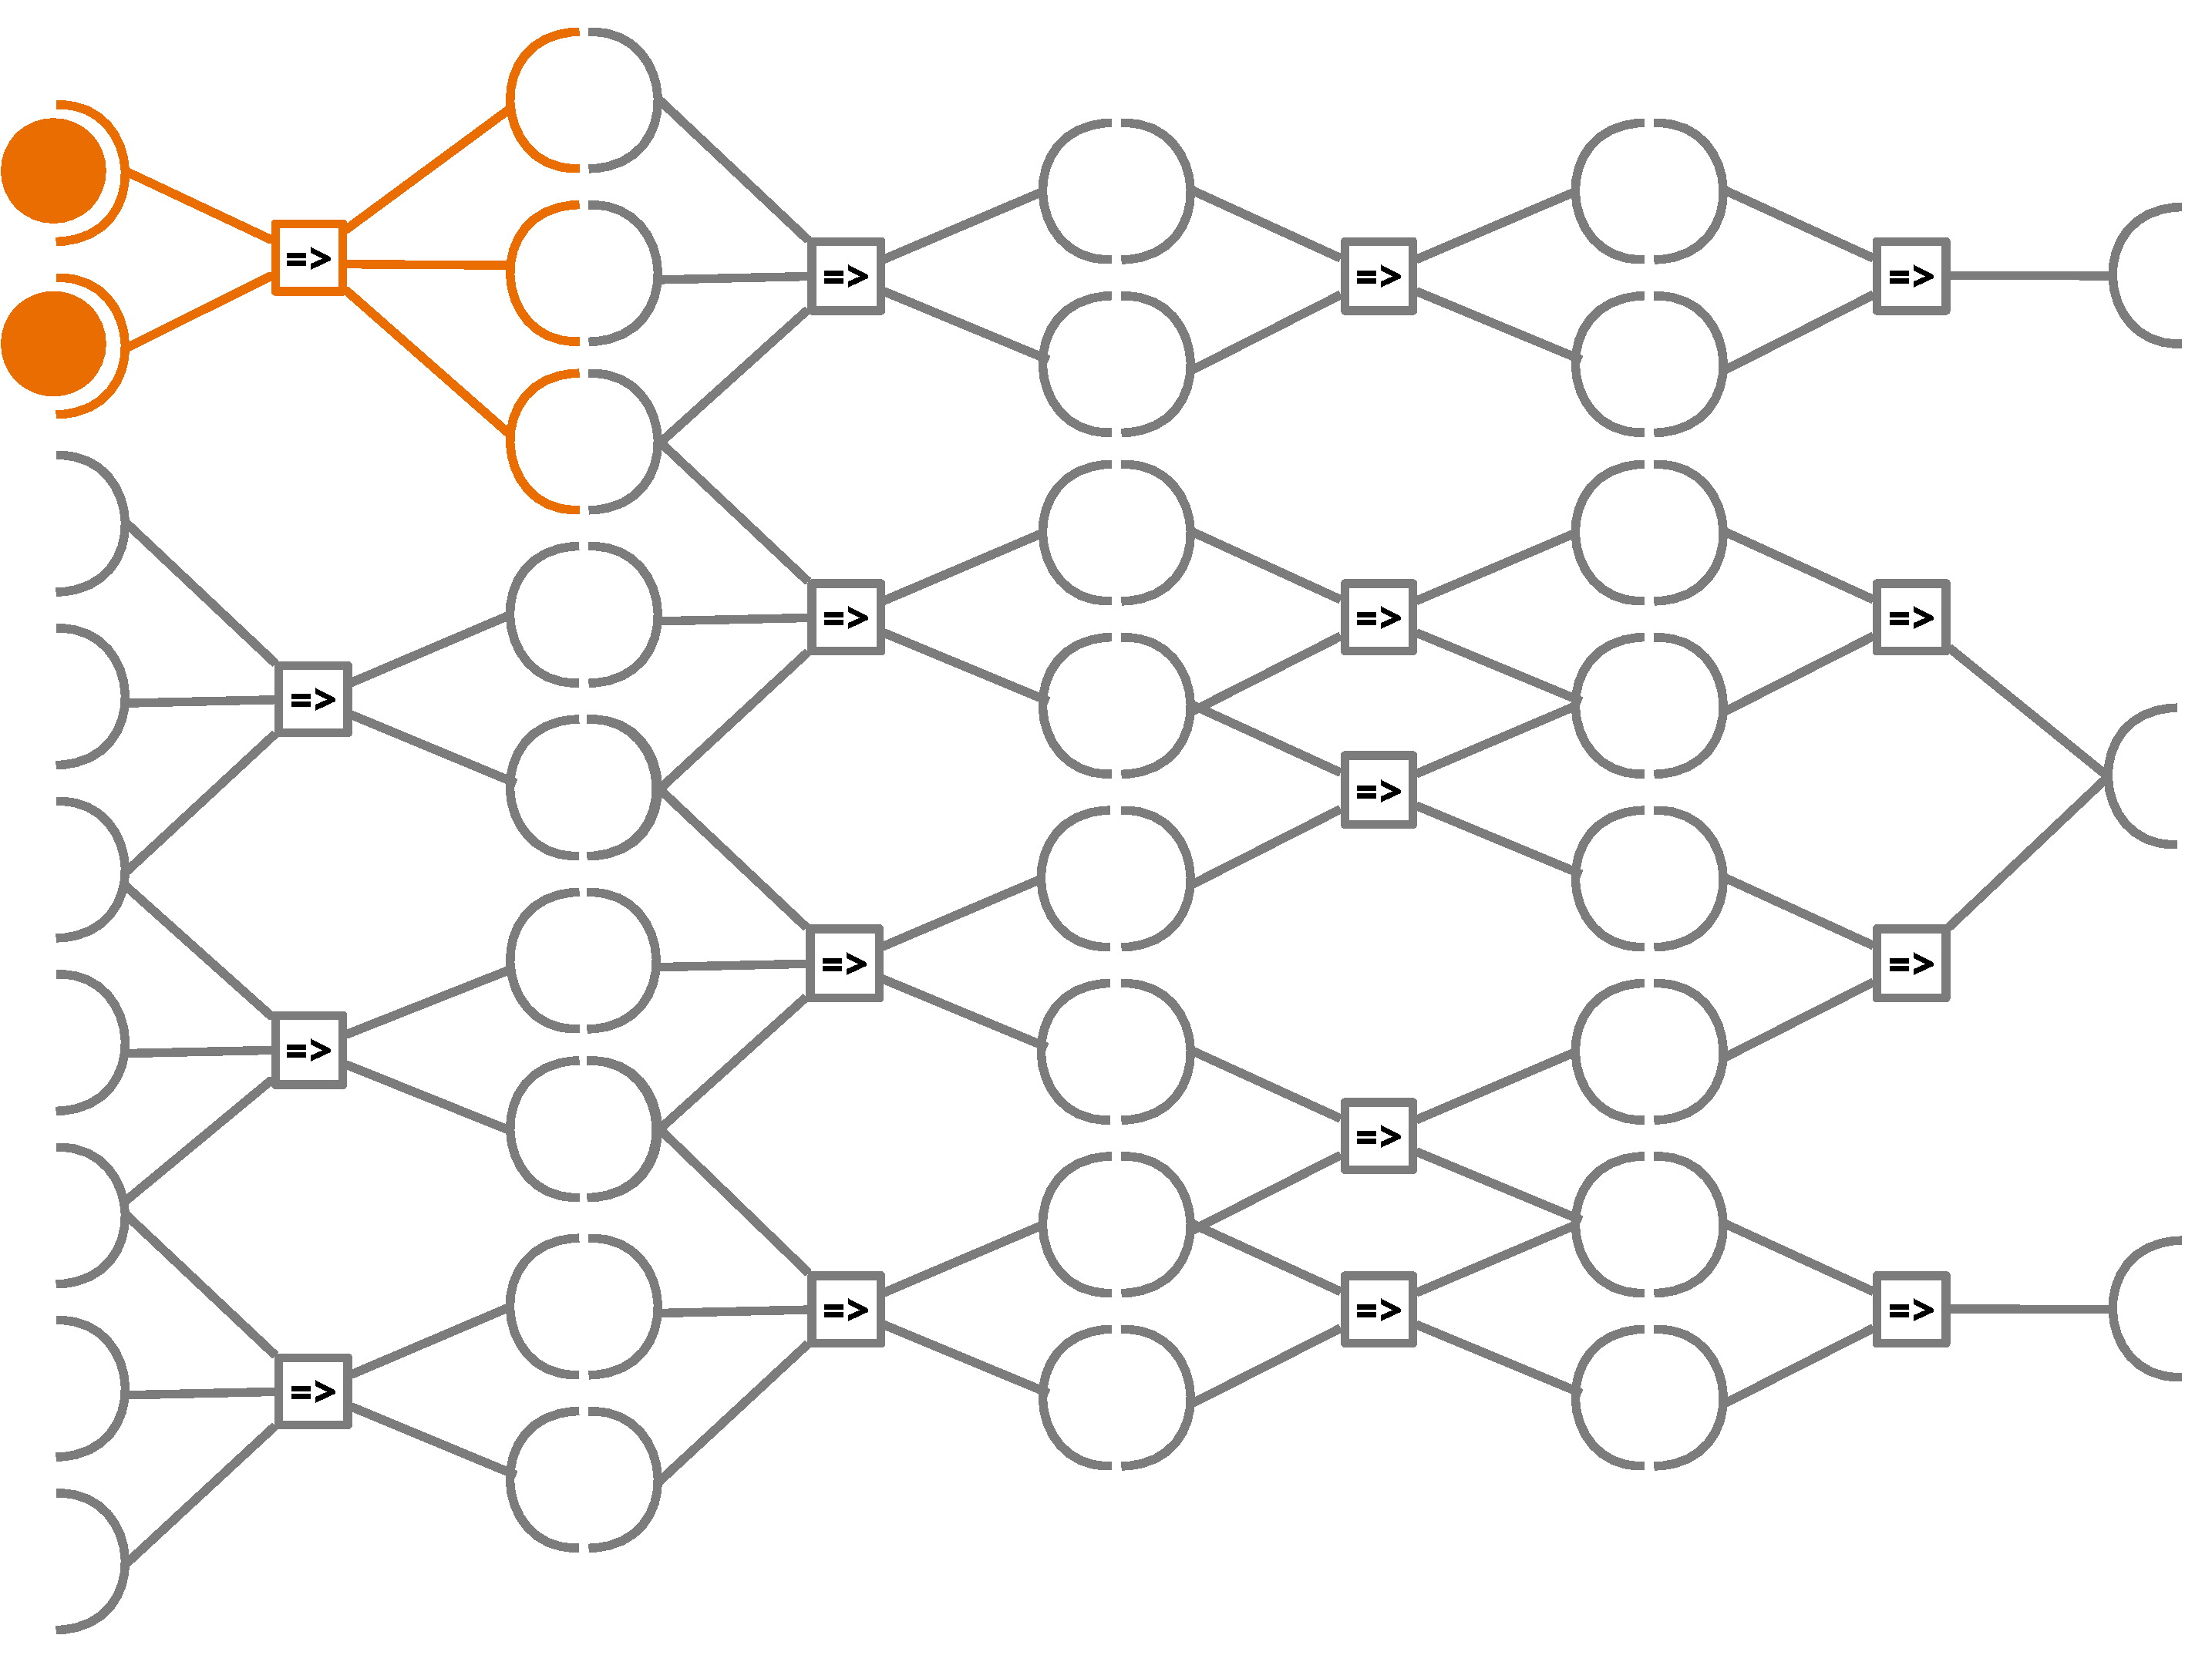
\includegraphics[width=0.7\linewidth]{Figures/rulesact-II}
  \end{center}
  It means that the rule
  gets instantiated, goes to the agenda, then\dots
\end{frame}

\begin{frame}
  \frametitle{Rule Hierarchy VI}
  \dots when fired it will probably alter the WM, allowing other
  branches in the path\dots
  \begin{center}
    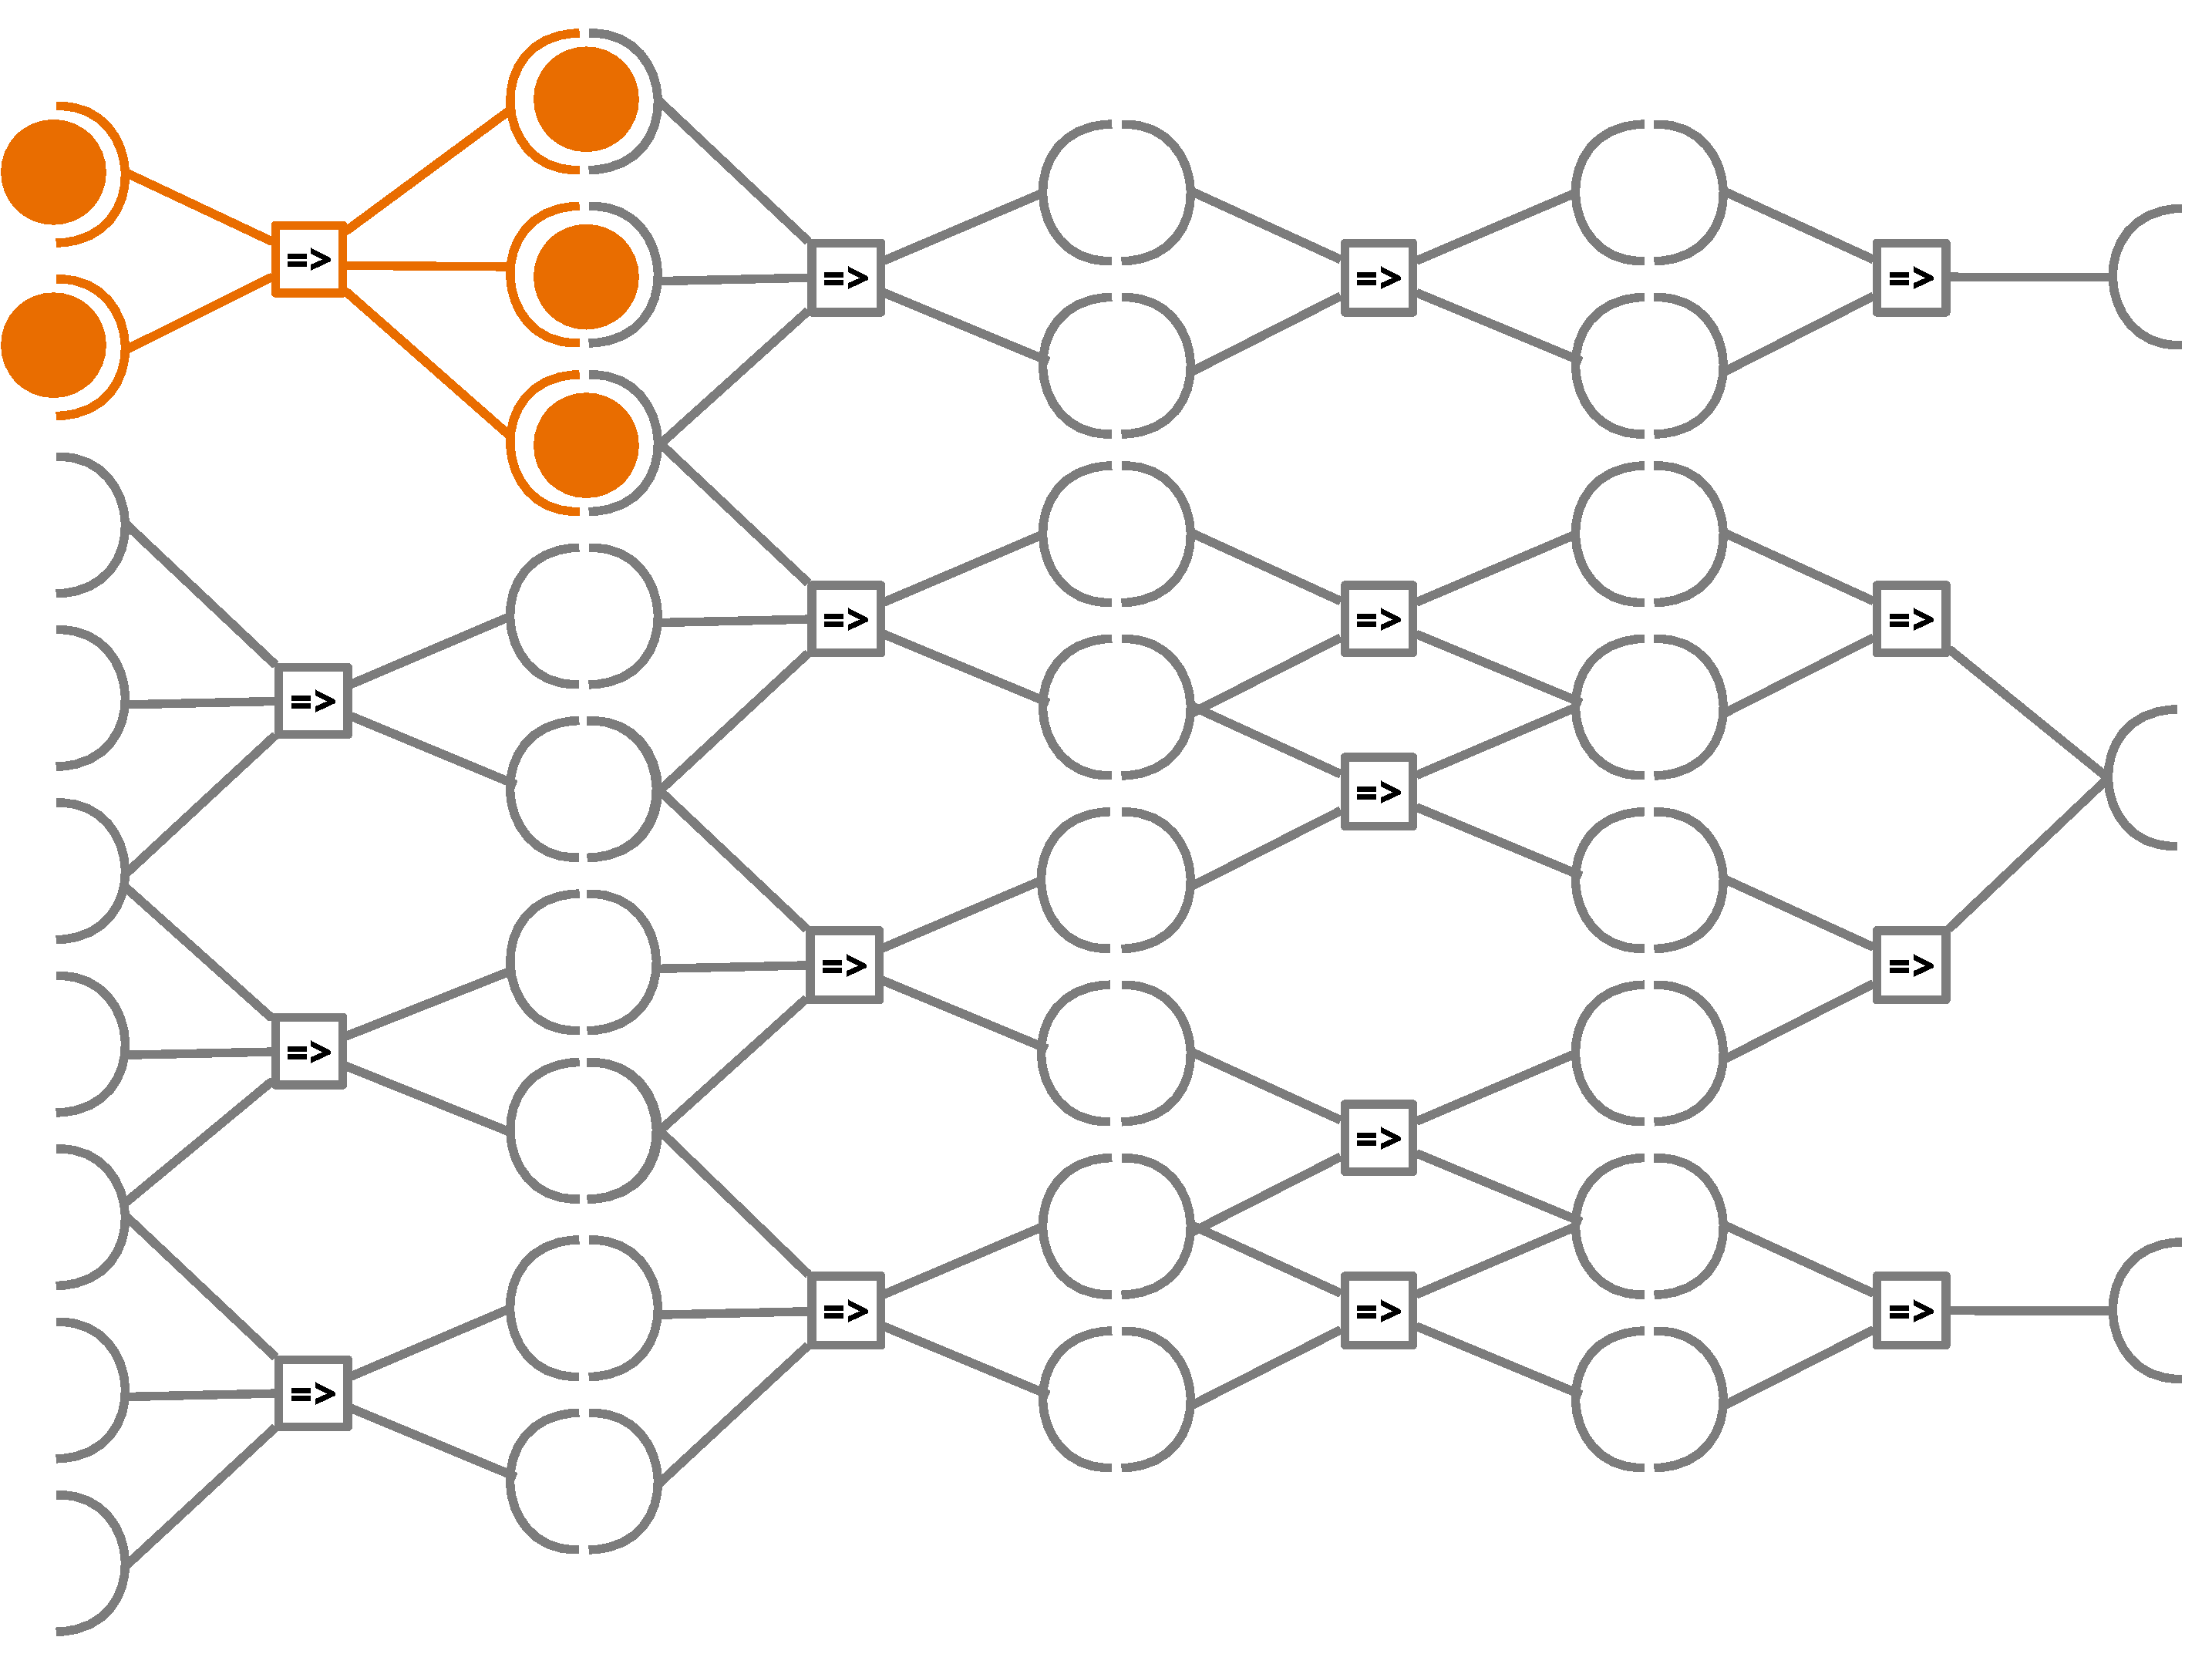
\includegraphics[width=0.7\linewidth]{Figures/rulesact-IIII}
  \end{center}
\end{frame}

\begin{frame}
  \frametitle{Rule Hierarchy VII}
  a full path is traversed when no more rules can get activated.
  \begin{center}
    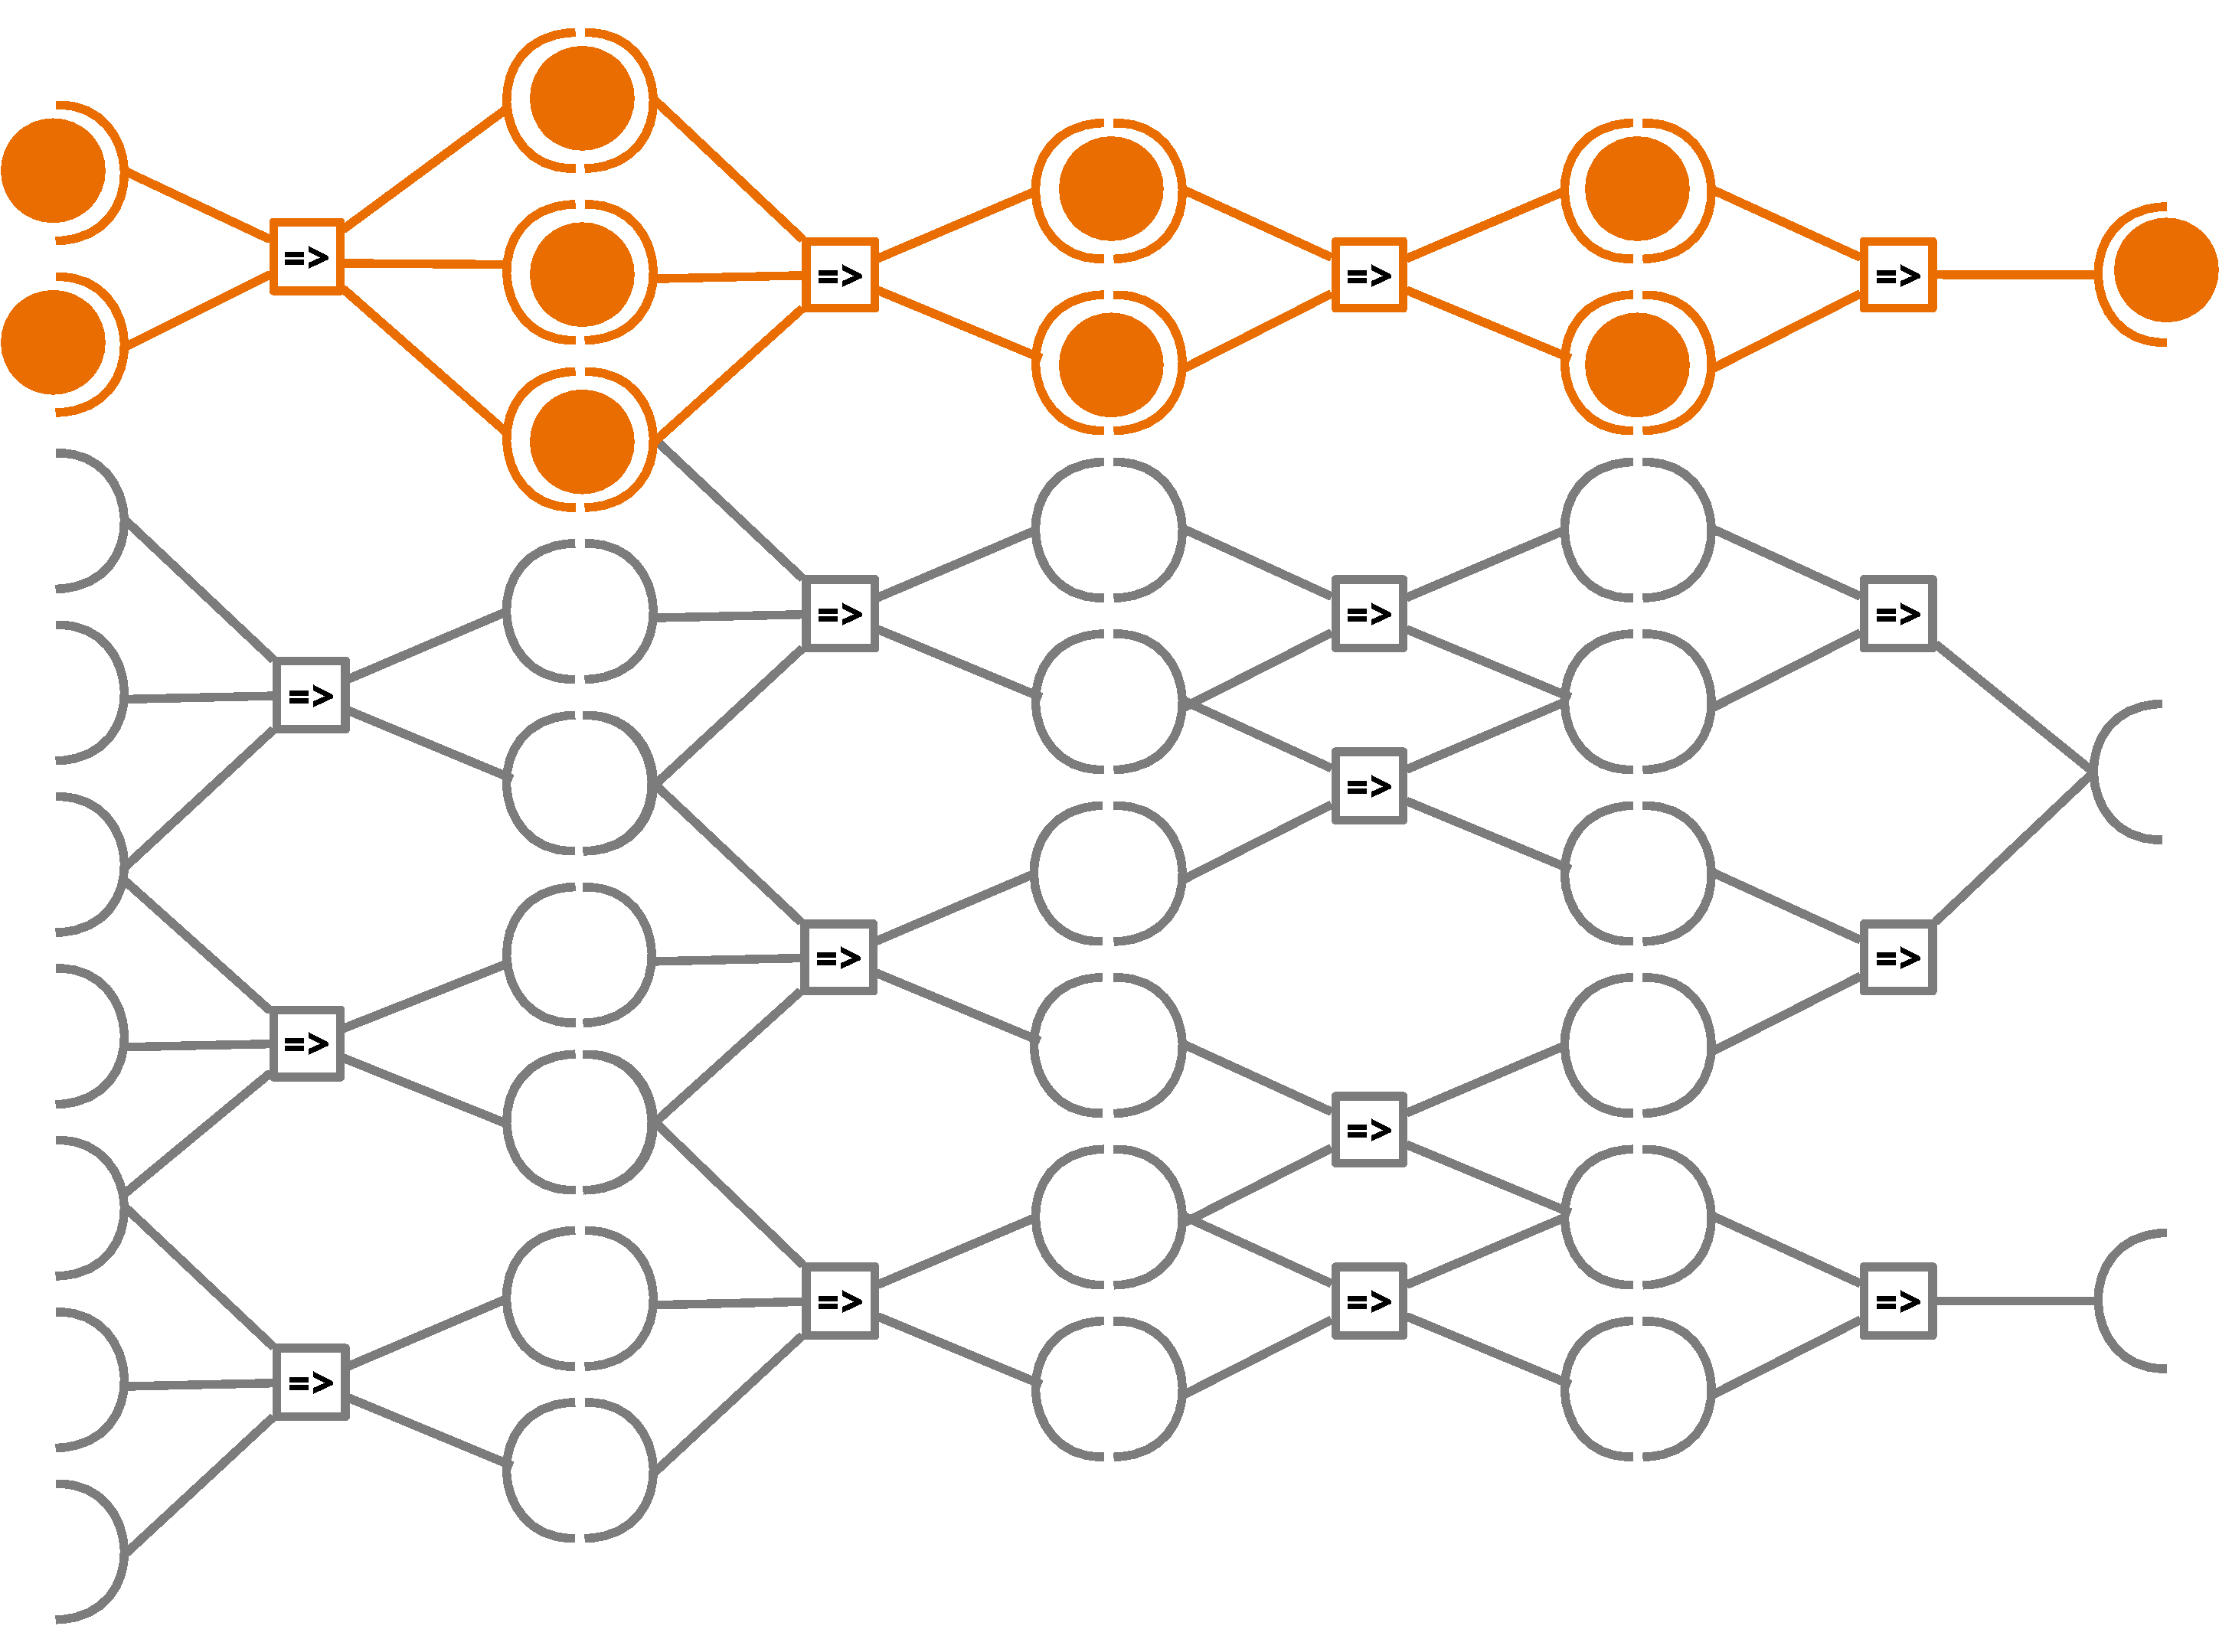
\includegraphics[width=0.7\linewidth]{Figures/rulesact-V}
  \end{center}
  The complexity and non linearity can be measured by the number of
  alternative paths\dots
\end{frame}

\begin{frame}
  \frametitle{Rule Hierarchy VIII}
  \begin{center}
    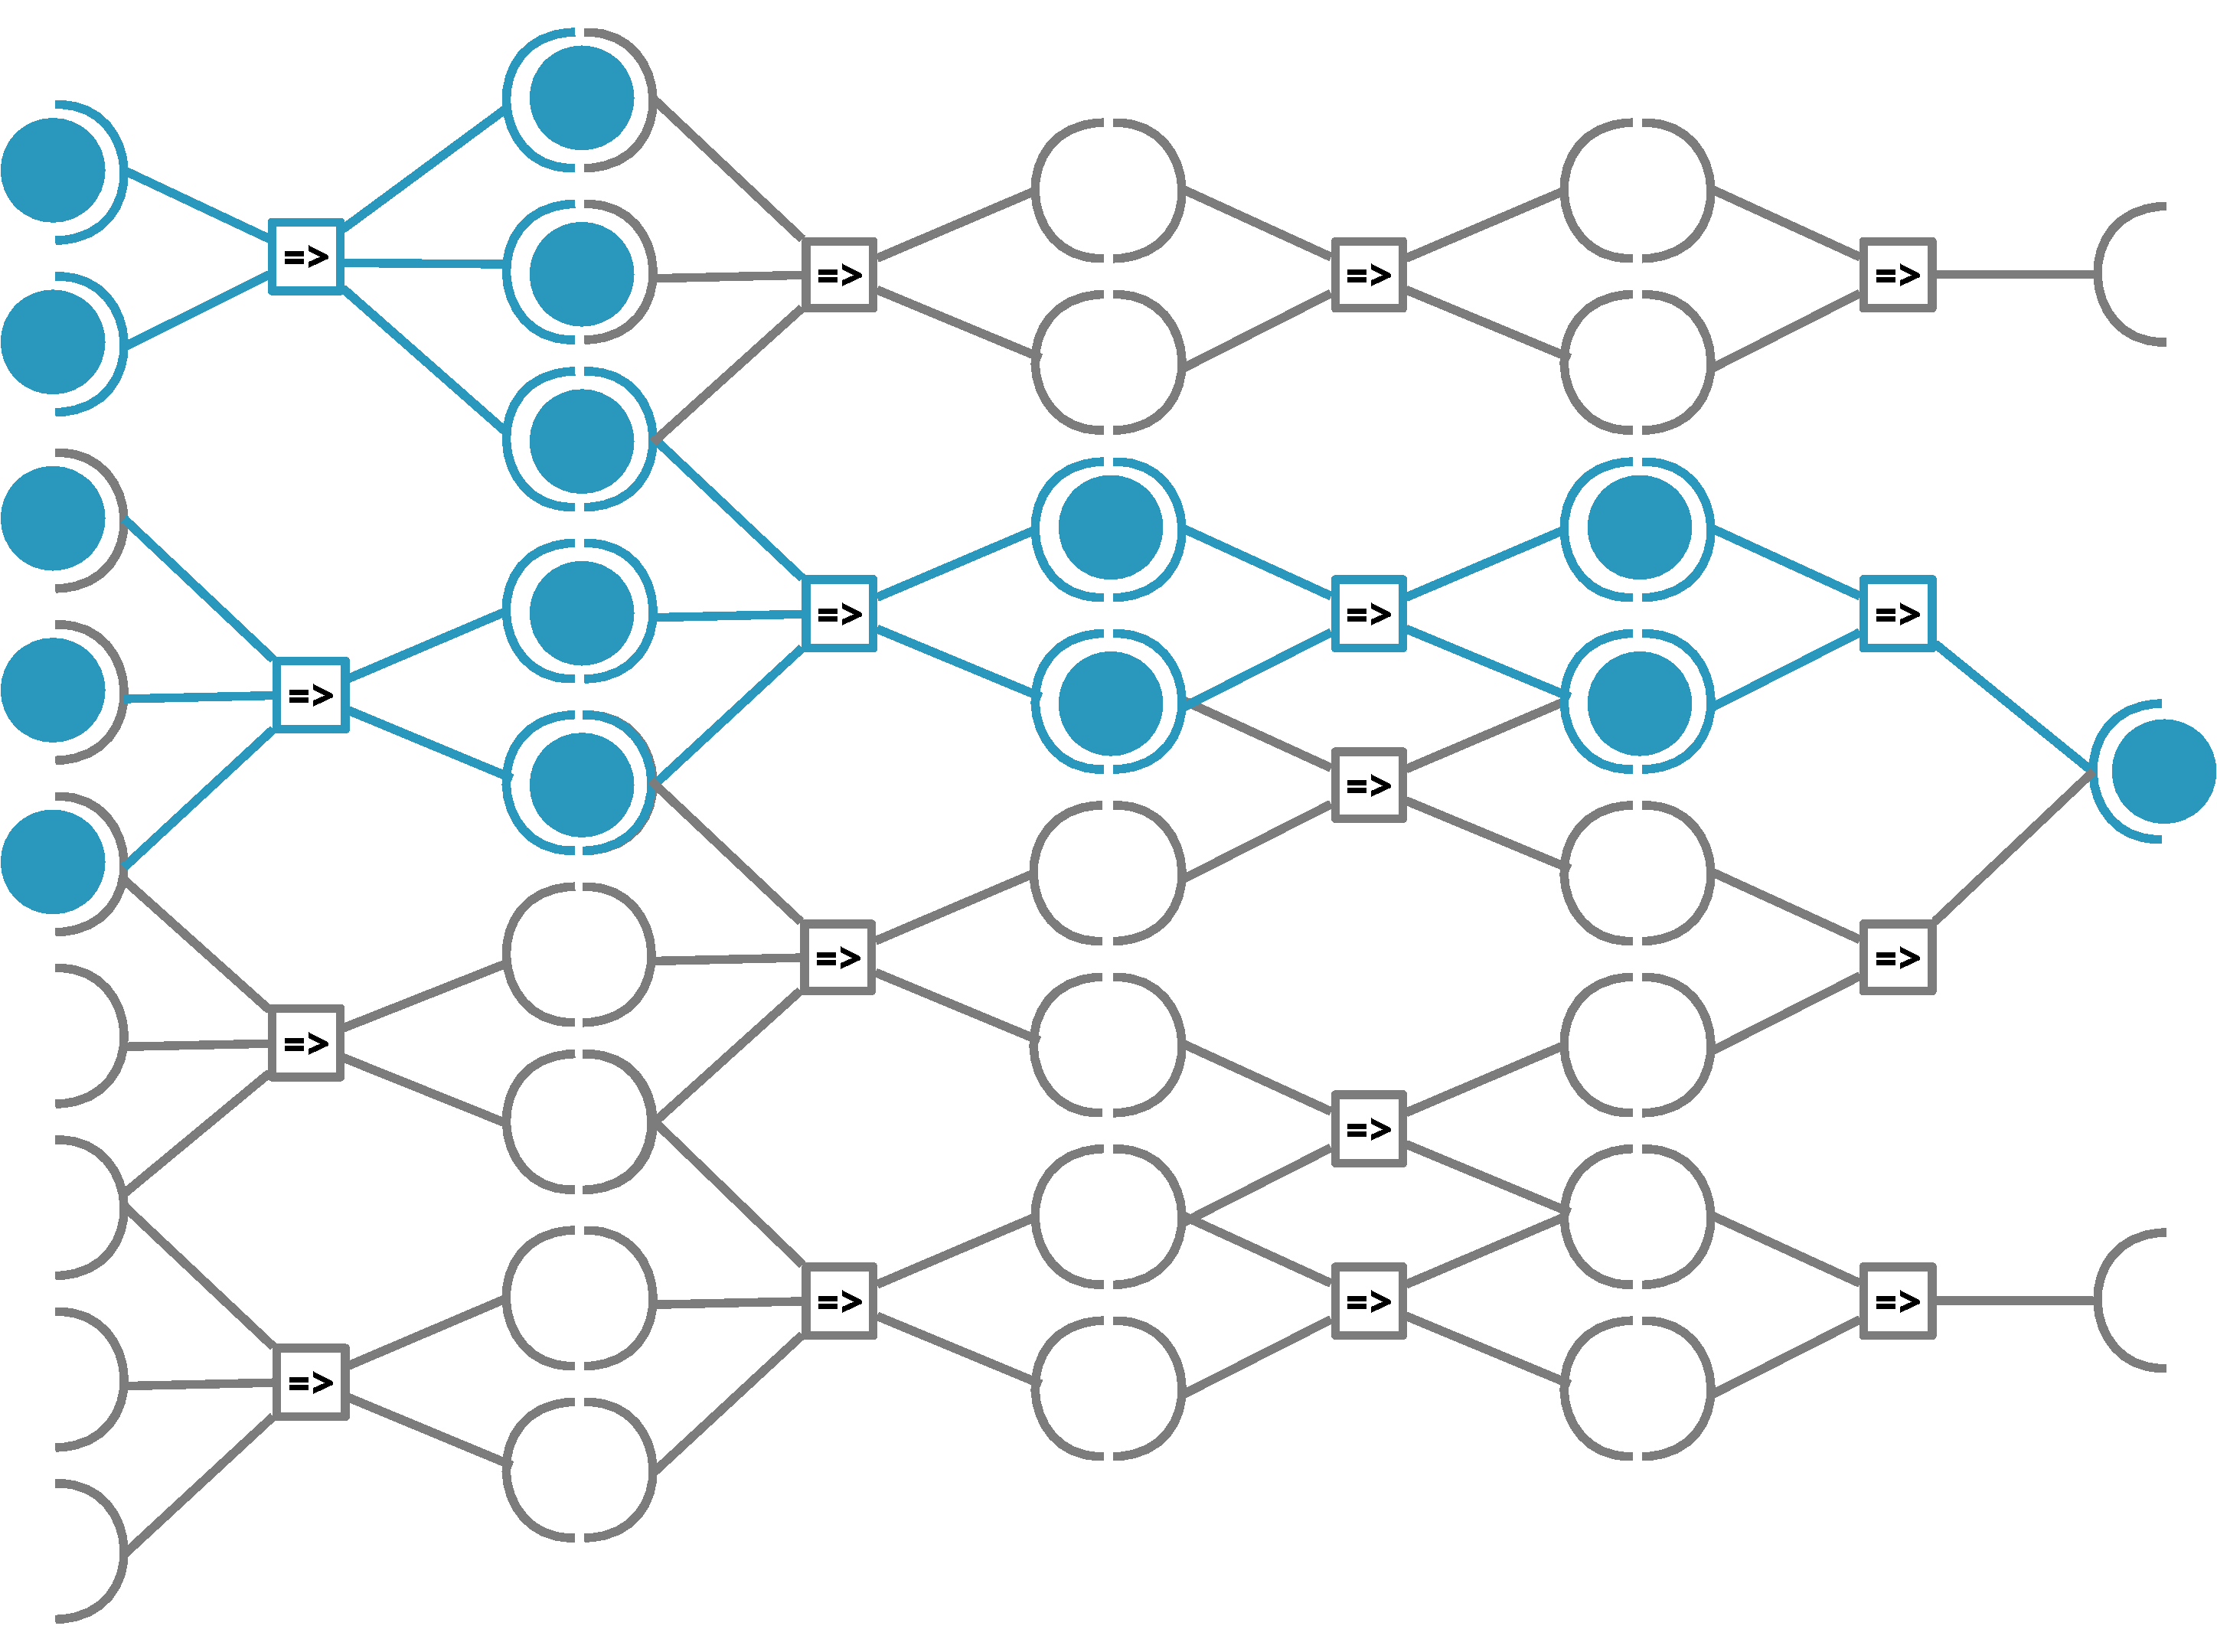
\includegraphics[width=0.7\linewidth]{Figures/rulesact-VI}
  \end{center}
  Now consider this as a single module. Repeat the process at a
  higher abstraction level.
\end{frame}

\begin{frame}[fragile]
  \frametitle{Randomizing order}
  Our naive conversation behaviour could be more banal if we could
  start the conversation from any possible rule.\par\bigskip
  We can achieve this by imposing a random conflict resolution
  strategy (all rules to ask questions shall have the same priority):
  \begin{clips-code}
    (clear)
    (set-strategy random)
    (load icterus.clp)
    (reset)
    (run)
  \end{clips-code}

  However, please note that a real diagnostic interview can start from
  every point, \emph{but then it is then guided by
  the partial diagnosed diseases and symptoms}. In order to do this we
have to introduce meta-rules\dots\par\bigskip

  \textbf{If} there is a symptom that can be asked that is characterizing a
  disease we could diagnose, \textbf{then} ask about that symptom
\end{frame}

% \begin{frame}
%   \frametitle{Coping with Uncertainty}
  
% \end{frame}

\begin{frame}[fragile]
  \frametitle{Revising Asserted Knowledge}
  If we assume each asserted symptom to be erroneously observed, we
  could provide a routine that lets you change the truth value for
  them all, calling inference again on the new WM.\par
  \begin{clips-code}
    Would you like to revise the diagnosis? (yes/y/no/n): yes
    Would you like to change some observed symptom?
    (1) recurrent-pain: TRUE
    (2) tired: TRUE
    (3) enlarged-liver: TRUE
    (4) yellowish-skin: TRUE
    ...
    (11) enlarged-spleen: TRUE
    (12) alcohol-abuse: TRUE
    (13) cholecyst-pain: TRUE
    (14) fever: TRUE
    Enter the symptom number or 'e' to return or 'h' to stop:
  \end{clips-code}

  Suppose you are setting yellowish-skin to FALSE, will the scleral
  icterus rule fire? \emph{what if scleral icterus has already been asserted before}? 
\end{frame}

\begin{frame}[fragile]
  \frametitle{Revising Asserted Knowledge}
  A simple, manual approach:
  \begin{clips-code}
    (deffunction get-all-facts-by-names ($?template-names)
        (bind ?facts (create$))
        (progn$ (?f (get-fact-list)) ;; this is a foreach
            (if (member$ (fact-relation ?f) $?template-names)
                then (bind ?facts (create$ ?facts ?f)))) ?facts)
    
    (deffunction change-symptom-by-index (?index)
        (bind ?f (nth ?index (get-all-facts-by-names symptom)))
        (modify ?f (observed (not (fact-slot-value ?f observed)))))

    (deffunction ask-to-change-symptom (?question)
        (printout t "Would you like to change some observed symptom?" crlf)
        (print-all-symptoms-status)
        (bind ?n (length$ (get-all-facts-by-names symptom)))
        (bind ?response (ask-question ?question (create$ (gen-int-list ?n) e h)))
        (switch ?response  (case h then (printout t "Halt" crlf) (halt))
                           (case e then (return)) 
                           (default (change-symptom-by-index ?response)
        (ask-to-change-symptom ?question))))
  \end{clips-code}
\end{frame}

\section{Searching}
{\setbeamertemplate{headline}{}
  \begin{frame}
    \sectionpage
  \end{frame}
}

\begin{frame}
  \frametitle{Search State Representation}
  We can represent the inference problem as the search in the space of
  possible diagnosed states.\par
  To implement a problem solver in CLIPS we have to model, for each
  problem\footnote{How could we model a \emph{general problem solver}?}:
  \begin{description}
  \item[\textbf{states}] that form our search space (e.g. problem configurations)
  \item[\textbf{transitions}] that allow to jump from one state to its
    neighbors, the next states (e.g. rules in a game)
  \item[\textbf{constraints}] eventually imposed on states (e.g. no
    repeated or illegal states) and to check for a state to be a solution
    \item[\textbf{search strategy}] that controls which transition to
      apply and which state to move on at each time
    \item[\textbf{explored tree}] representing the states explored so far
  \end{description}
\end{frame}

\begin{frame}
  \frametitle{A tentative implementation}
  The simplest implementation we can try relies on the direct
  exploitation of the constructs that CLIPS offers, using in a
  non-transparent way its inference cycle\par\bigskip
  To be more precise we would have:
  \begin{description}
  \item[\textbf{states}] as facts in the current configuration of the WM.
  \item[\textbf{transitions}] encoded directly as CLIPS rules with the
    same priority
  \item[\textbf{constraints}] as constrained pattern in the LHS of
    transitions (e.g. the \textsf{not} logical operator). Some rules
    can be explicitly used for solution states
  \item[\textbf{search strategy}] directly relying on CLIPS conflict
    resolution strategy
  \item[\textbf{explored tree}] building it by some other facts as we
    proceed
  \end{description}
  Even though it lacks flexibility and constraints us in many ways, we
  will explore a use case by implementing a very simple game before moving forward. 
\end{frame}
\begin{frame}
  \frametitle{8-Puzzle}
  The \href{http://en.wikipedia.org/wiki/15_puzzle}{8-puzzle} game is
  one of the earliest games exploited in AI. Numbered tiles, from 1 to
  8, are placed on a $3\times3$ grid.\par Starting from an initial grid
  configuration the objective is to reach a final state in which all
  tiles are ordered numerically with the last one left empty.\par
  The allowed moves consist in exchange the position of the the empty
  tile with one of its (at most) four neighbors.
  \begin{table}
    \setlength\tabcolsep{2pt}
    \centering
    \tiny
    \begin{tabular}{c c c c }
      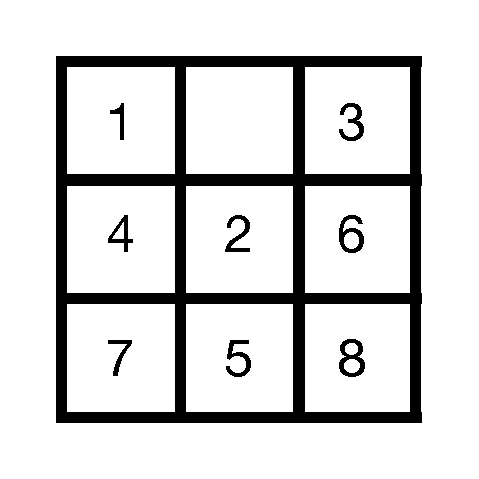
\includegraphics[width=70pt]{Figures/8-puzzle-4}
      & 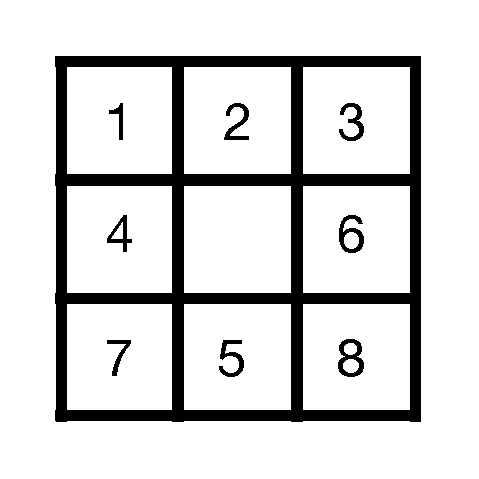
\includegraphics[width=70pt]{Figures/8-puzzle-3}
      & 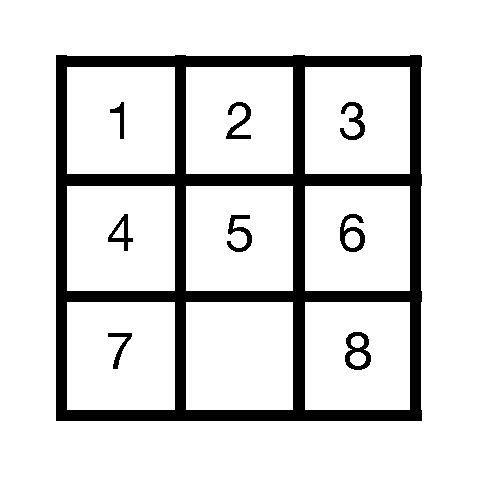
\includegraphics[width=70pt]{Figures/8-puzzle-2}
      & 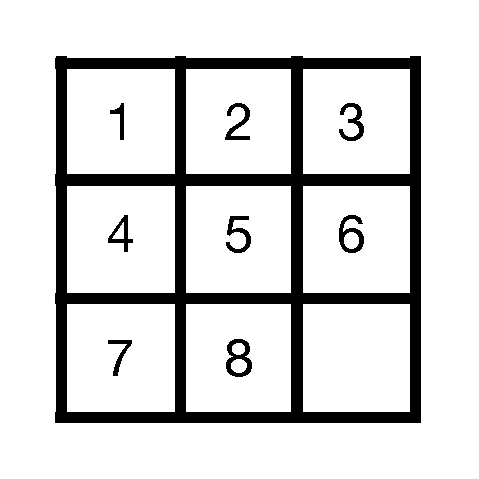
\includegraphics[width=70pt]{Figures/8-puzzle-1}\\
    \end{tabular}
  \end{table}
  At this point of the course you should be pretty familiar with this game.
\end{frame}

\begin{frame}[fragile]
  \frametitle{8-Puzzle: Facts and Rules}
  Concerning states we can represent a grid configuration with a
  single fact. The information to be stored concerns \emph{the numbered
  positions} and \emph{the actual value} in them. For instance, we can use a special number
  like $-1$ to represent the empty tile value.\par\bigskip

  Even if inefficiently we can take advantage of the WM
  by simply asserting and never retracting (remind assertion and
  refraction properties).\par\bigskip

  We can have each rule modeling a single possible empty cell movement
  (24 rules total), something like:\par\bigskip

  \textbf{If} the grid has $X_1$ in the 1st position, -1 in the 2nd, $X_3$ in the
  third, $X_4$ in the fourth, $X_5$ in the fifth, \dots, \textbf{then} the new
  grid will be:  $X_1$ in the 1st position, $X_5$ in the 2nd, $X_3$ in the
  third, $X_4$ in the fourth, -1 in the fifth,\dots\par\bigskip

  We could reduce the number of rules by exploiting functional abstraction.\par

  
  
  
\end{frame}

\begin{frame}[fragile]
  \frametitle{8-Puzzle: Constraints and Strategy}
  Avoiding loops is done by the WM use we are doing and by enforcing
  to match only rules leading to unseen configurations.\par
  Refraction helps, but we need to avoid even to trigger rules that
  would assert and already asserted state.\par

  One possible solution is to put a constraint as a pattern in the LHSs:\par\bigskip

  \textbf{If} the grid has $X_1$ in the 1st position, -1 in the 2nd, $X_3$ in the
  third, $X_4$ in the fourth, $X_5$ in the fifth, \dots, \textbf{AND}
  there is \emph{not} $X_1$ in the 1st position, $X_5$ in the 2nd, $X_3$ in the
  third, $X_4$ in the fourth, -1 in the fifth\dots, \textbf{then} the new
  grid will be:  $X_1$ in the 1st position, $X_5$ in the 2nd, $X_3$ in the
  third, $X_4$ in the fourth, -1 in the fifth,\dots\par\bigskip

  The search strategy can be demanded to CLIPS by enforcing all rules
  to have the same salience and by employing the \textsf{breadth} or
  \textsf{depth} conflict resolution strategy.
  \begin{clips-code}[numers=none]
    (set-strategy depth)
  \end{clips-code}
  What is, for this particular problem, the best strategy to employ? why?\par

\end{frame}

\begin{frame}
  \frametitle{8-Puzzle: Constraints and Search Tree}
  As a last constraint we need rules to check for a state to be the
  final one (solution). This is simply done like in the previous
  fashion.\par\bigskip
  
  To build a search tree we can store its edge information as facts
  containing information about the two configurations of the
  world, the parent and child grids.\par\bigskip

  After a solution has been found we have to crawl back from that
  state to the root. To do this we need a simple rule that searches
  for a state matching for the parent attribute in our edge facts\par\bigskip

  

  
\end{frame}

\begin{frame}[fragile]
  \frametitle{Exercise}
  Implement such a problem solver for the 8-puzzle.\par\bigskip
  
  \textbf{Hint 1}:\par
  While programming apply a debugging strategy, inspect the WM after
  each activated rule execution. Moreover, keep track of strategy
  resolution by printing to stout the state that activates a rule and
  the one that the rule asserts.\par\bigskip
  
  \textbf{Hint 2}:\par
  To set the strategy and maybe constants use another file to by
  loaded with the \textsf{batch} function.\par\bigskip

  \textbf{Hint 3}:\par
  For the tree representation you can use something like this for
  edges, containing simply the fact addresses (pointers):
  \begin{clips-code}[numbers=none]
    (deftemplate move
        (slot parent (type FACT-ADDRESS) (default ?NONE))
        (slot next (type FACT-ADDRESS) (default ?NONE)))
  \end{clips-code}
      
\end{frame}

\begin{frame}[fragile]
  \frametitle{8-Puzzle: a possible solution I}
  A very simple (and verbose) representation for states as facts:
  \begin{clips-code}[numbers=none]
    (deftemplate 8-puzzle
        (slot one (type INTEGER) (default ?NONE))
        (slot two (type INTEGER) (default ?NONE))
        (slot three (type INTEGER) (default ?NONE))
        (slot four (type INTEGER) (default ?NONE))
        (slot five (type INTEGER) (default ?NONE))
        (slot six (type INTEGER) (default ?NONE))
        (slot seven (type INTEGER) (default ?NONE))
        (slot eight (type INTEGER) (default ?NONE))
        (slot nine (type INTEGER) (default ?NONE)))

    (deftemplate move
        (slot parent (type FACT-ADDRESS) (default ?NONE))
        (slot next (type FACT-ADDRESS) (default ?NONE)))
 
    (deffacts initial-board
        (8-puzzle (one 1) (two 2) (three 3) (four 4) (five -1) (six 6)
                  (seven 7) (eight 5) (nine 8)))
  \end{clips-code}
\end{frame}

\begin{frame}[fragile]
  \frametitle{8-Puzzle: a possible solution II}
  An equally simple (and verbose) formulation for the rules:
  \begin{clips-code}[numbers=none]
    (defrule from-one-to-two
        ?s <-(8-puzzle (one -1) (two ?T) (three ?H) 
                       (four ?F) (five ?I) (six ?S) 
                       (seven ?E) (eight ?G) (nine ?N))
        (not (8-puzzle (one ?T) (two -1) (three ?H)
                       (four ?F) (five ?I)  (six ?S) 
                       (seven ?E) (eight ?G) (nine ?N)))
        =>
        (bind ?n (assert (8-puzzle (one ?T) (two -1) (three ?H)
                                   (four ?F) (five ?I) (six ?S) 
                                   (seven ?E) (eight ?G) (nine ?N))))
        (print-boards ?s ?n)
        (printout t "Moved from one to two" crlf)
        (assert (move (parent ?s) (next ?n)))
        (yes-or-no-halt))
      \end{clips-code}

  The check to not activate a rule leading to an already seen
  configuration is embedded as a \textsf{not} CE in the LHS.
\end{frame}

\begin{frame}[fragile]
  \frametitle{8-Puzzle: a possible solution III}
  To detect if we have reached a final configuration, we can employ a
  fixed LHS rule:
  \begin{clips-code}[numbers=none]
    (defrule found-solution
        (declare (salience ?*highest-priority*))
        ?s <- (8-puzzle (one 1) (two 2) (three 3)
                        (four 4) (five 5) (six 6) 
                        (seven 7) (eight 8) (nine -1))
        (move (parent ?p) (next ?s))
        =>
        (print-boards ?s ?s)
        (assert (moves ?p ?s))
        (printout t "FOUND solution" crlf))
      \end{clips-code}

   While, to govern the search strategy we have to set the conflict
   resolution strategy in CLIPS, which can be done in a batch file:
   \begin{clips-code}[numbers=none]
     (clear)
     (set-strategy breadth)
     (load 8_puzzle.clp)
     (reset)
     (run)
 \end{clips-code}
\end{frame}

\begin{frame}[fragile]
  \frametitle{8-Puzzle: a possible solution IV}
  To retrieve the path leading to the final correct configuration, we
  can use also other rules, collecting back the \textsf{move} facts a create a
  multifield \textsf{moves} fact which (we can print at the end).
  \begin{clips-code}[numbers=none]
    (defrule get-solution-path
        (declare (salience ?*highest-priority*))
        ?m <- (moves ?last-move $?other-moves)
        ?k <- (move (parent ?previous) (next ?last-move))
        =>
        (retract ?m ?k)
        (assert (moves ?previous ?last-move $?other-moves)))

    (defrule print-solution-path
        (declare (salience ?*highest-priority*))
        ?m <- (moves ?last-move $?other-moves)
        (not (move (parent ?previous) (next ?last-move))) ;; this is the root
        =>
        (printout t "Found a solution" crlf)
        (print-board-moves ?m)
        (halt))
  \end{clips-code}
\end{frame}

\begin{frame}
  \frametitle{Pros\&Cons}
  What \textbf{\emph{we gain for free}} is CLIPS inference routines and constructs,
  i.e. we do not have to implement a breadth first search or the
  neighbor space generation by ourselves (we just describe how they are generated
  via transition rules).\par\bigskip
  
  However, \emph{we cannot explore the search space in a more sophisticated way}.\par
  
  If we use CLIPS conflict resolution strategy for free, we cannot
  assign different priorities to rules. Neither it is possible to
  implement other search techniques like best-first search, $A^{*}$,
  and so on. We could implement the Manatthan distance heuristic
  score as a function, but we would have no way to embed its
  evaluation on the pairs of states.\par\bigskip

  A higher level representation for transition rules and states is
  needed.
\end{frame}

\begin{frame}
  \frametitle{Cannibals and Missionaries (CaM)}
  We have an initial equal number $N$ of cannibals and missionaries on one
  shore of a river. There is one boat that can transport at most
  $k$ people at a time from one side to the other. We start with $2N$
  people on one shore and we have to move all to the other. considering that, at each time,
  on both shore and on the boat, the number of missionaries shall be
  equal or greater than that of cannibals.\par
  Supposing $N=3$ and $k=2$ a possible state search space is:\par\bigskip
  \begin{center}
    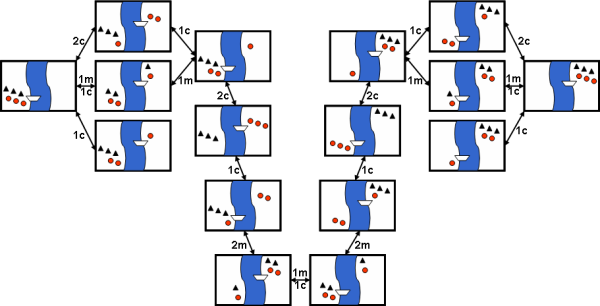
\includegraphics[width=0.7\textwidth]{Figures/cam}
  \end{center}

\end{frame}

\begin{frame}[fragile]
  \frametitle{CaM: State formulation I}
  To be able to govern more the search, we need to embed in the state
  conceptualization some references to the current search advancement
  (e.g. depth, references to the parent state,\dots)\footnote{This
  code is taken from Giarratano's and Riley's book}: 
  \begin{clips-code}[numbers=none]
    (deftemplate MAIN::status 
        (slot search-depth (type INTEGER) (range 1 ?VARIABLE))
        (slot parent (type FACT-ADDRESS SYMBOL) (allowed-symbols no-parent))
        (slot shore-1-missionaries (type INTEGER) (range 0 ?VARIABLE))
        (slot shore-1-cannibals (type INTEGER) (range 0 ?VARIABLE))
        (slot shore-2-missionaries (type INTEGER) (range 0 ?VARIABLE))
        (slot shore-2-cannibals (type INTEGER) (range 0 ?VARIABLE))
        (slot boat-location (type SYMBOL) (allowed-values shore-1 shore-2))
        (slot last-move (type STRING)))   
  \end{clips-code}
  as well as taking into account the boat position and number of
  missionaries and cannibals on both shores.
      
\end{frame}

\begin{frame}[fragile]
  \frametitle{Modular Programming}
  In CLIPS it is possible to define different modules, each one with
  its deftemplated facts, rules, function, global variables (everything that can be
  build with a \textsf{def} construct).\par
  To define a module, use the construct \textsf{defmodule}.\par
  To specify the name of a module as a \textbf{\emph{namespace}}, one shall use the scope
  operator \textsf{::} (like in C++)\par\bigskip
  One module can import from others the constructs it needs to
  operate. Image we use a MAIN module to represent the state and the
  rules to operate on them, we could use a CONSTRAINT module for rules
  checking illegal states and a module SOLUTION for getting the path
  from the root of the search tree to the final configuration
  state. To import the \textsf{status} template in the CONSTRAINT
  module we could write:
  \begin{clips-code}[numbers=none]
    (defmodule CONSTRAINTS 
       (import MAIN deftemplate status))
  \end{clips-code}

  The switch among modules can be governed by the \textsf{focus}
  property (see rules later).
  \begin{clips-code}[numbers=none]
    
  \end{clips-code}
\end{frame}

\begin{frame}[fragile]
  \frametitle{Focus-Stack}
  In order to manage the modules of a program CLIPS maintains a stack
  of module references, the \textsf{focus-stack}. The module at the top of the
  focus-stack is active; all the others are dormant.\par
  The rules in a module can contain actions that modify the contents of the
  focus-stack and thus force the activation of other
  modules.\par\bigskip

  If the rule of a module is declared auto-focus, by using the special
  pattern
  \begin{clips-code}[numbers=none]
    (declare (auto-focus TRUE))
  \end{clips-code}
  then the module will be automatically activated and inserted at the top of the
  \textsf{focus-stack} when the rule becomes instantiated.\par
  Note that this creates an effect similar to that of putting a very
  high priority on that rule.\par\bigskip

  This way not only we can \emph{divide} rules into modules (doing different
  tasks), but we can also \emph{govern} their activation (by determining
  their modules activation).
\end{frame}

\begin{frame}[fragile]
  \frametitle{CaM: State formulation II}
  We can represent the initial status as shown in the previous image
  with a \textsf{deffacts} construct.
  \begin{clips-code}[numbers=none]
    (deffacts MAIN::initial-positions
         (status (search-depth 1) 
                 (parent no-parent)
                 (shore-1-missionaries 3)
                 (shore-2-missionaries 0)
                 (shore-1-cannibals 3)
                 (shore-2-cannibals 0)
                 (boat-location shore-1)
                 (last-move "No move.")))

    (deffacts boat-information
        (boat-can-hold 2))
  \end{clips-code}
\end{frame}

\begin{frame}[fragile]
  \frametitle{CaM: Generate \& Test I}
  To search the state space we can adopt a \textbf{\emph{generate \&
      test}} approach: that is, we generate (assert) all the possible
  \emph{syntactical} states by moving one or more cannibals and/or
  missionaries from one shore to the other. After the states have been
  generated, we can use other rules to prune (retract) those that are
  illegal, for instance statuses where the number of cannibals exceeds
  that of missionaries:
  \begin{clips-code}[numbers=none]
    (defrule CONSTRAINTS::cannibals-eat-missionaries
         (declare (auto-focus TRUE))
         ?node <- (status (shore-1-missionaries ?s1m)
         (shore-1-cannibals ?s1c)
         (shore-2-missionaries ?s2m)
         (shore-2-cannibals ?s2c))
         (test (or (and (> ?s2c ?s2m) (<> ?s2m 0))
                   (and (> ?s1c ?s1m) (<> ?s1m 0))))
         =>
         (retract ?node))
  \end{clips-code}
  The property \textsf{auto-focus} tells CLIPS to apply inference in
  the referenced module as soon as it is possible to do so. In this
  case if this rule gets activated by a status, than the focus of
  execution will switch to the CONSTRAINTS module.
\end{frame}

\begin{frame}[fragile]
  \frametitle{CaM: Generate \& Test II}
  To generate all the states we can use just two rules that, for each
  shore, will calculate all the possible movements. (See the attached
  script for the full code)
  \begin{clips-code}[numbers=none]
    (defrule shore-1-move 
        ?node <- (status (search-depth ?num) 
                         (boat-location shore-1)
                         (shore-1-missionaries ?s1m)
                         (shore-1-cannibals ?s1c)
                         (shore-2-missionaries ?s2m)
                         (shore-2-cannibals ?s2c))
                         (boat-can-hold ?limit)
        =>
        (bind ?max-missionaries (min ?s1m ?limit))
        (loop-for-count (?missionaries 0 ?max-missionaries)
                        ...
                        (loop-for-count (?cannibals ?min-cannibals ?max-cannibals)
                                        (duplicate ?node (search-depth =(+ 1 ?num))
                                                         (parent ?node)
                                                         ...))))
  \end{clips-code}
\end{frame}

\begin{frame}
  \frametitle{CaM: exercise}
  Given the incomplete script for this problem, complete the
  CONSTRAINTS module by implementing the following rules:
  \begin{itemize}
  \item A rule to consider illegal all the states that have been
    generated over a certain depth limit
  \item A rule to check whether a state has already been visited
    before (hint, given this formulation, such a state would have all
    attributes equal to an already asserted state, for the exception of...)
  \end{itemize}\bigskip
 Implement a SOLUTIONS module that, like in the icterus case, is able
 to retrieve the paths from the root to a solution (final
 state). Hint: let the last slot of a status be its printed proxy.\par
 Keep in mind to import all the constructs that you need from other modules.\par\bigskip

 Extend the module to find all the possible solutions.
\end{frame}
% \begin{frame}[fragile]
%   \frametitle{State formulation}
%   % To be able to govern more the search, we need to embed in the state
%   % conceptualization some references to the current search advancement
%   % (e.g. depth, references to the parent state,\dots)\footnote{This
%   %   code is taken from Giarratano\'s and Riley\'s book}:
%   % \begin{clips-code}
%   %   (deftemplate MAIN::status 
%   %       (slot search-depth (type INTEGER) (range 1 ?VARIABLE))
%   %       (slot parent (type FACT-ADDRESS SYMBOL) (allowed-symbols no-parent))
%   %       (slot shore-1-missionaries (type INTEGER) (range 0 ?VARIABLE))
%   %       (slot shore-1-cannibals (type INTEGER) (range 0 ?VARIABLE))
%   %       (slot shore-2-missionaries (type INTEGER) (range 0 ?VARIABLE))
%   %       (slot shore-2-cannibals (type INTEGER) (range 0 ?VARIABLE))
%   %       (slot boat-location (type SYMBOL) (allowed-values shore-1 shore-2))
%   %       (slot last-move (type STRING)))
%   %     \end{clips-code}
%    as well as taking into account the boat position and number of
%    missionaries and cannibals on both shores.   
%  \end{frame}

 
 % \begin{frame}[fragile]
 %   \frametitle{Rules to generate states}
 %   \begin{clips-code}[numbers=none]
 %     (defrule MAIN::shore-1-move 
 %         ?node <- (status (search-depth ?num) 
 %                          (boat-location shore-1)
 %                          (shore-1-missionaries ?s1m)
 %                          (shore-1-cannibals ?s1c)
 %                          (shore-2-missionaries ?s2m)
 %                          (shore-2-cannibals ?s2c))
 %         (boat-can-hold ?limit)
 %         =>
 %         (bind ?max-missionaries (min ?s1m ?limit))
 %         (loop-for-count (?missionaries 0 ?max-missionaries)
 %         (bind ?min-cannibals (max 0 (- 1 ?missionaries)))
 %         (bind ?max-cannibals (min ?s1c (- ?limit ?missionaries)))
 %         (loop-for-count (?cannibals ?min-cannibals ?max-cannibals)
 %             (duplicate ?node (search-depth =(+ 1 ?num))
 %                                             (parent ?node)
 %                                             (shore-1-missionaries (- ?s1m ?missionaries))
 %                                             (shore-1-cannibals (- ?s1c ?cannibals))
 %                                             (shore-2-missionaries (+ ?s2m ?missionaries))
 %                                             (shore-2-cannibals (+ ?s2c ?cannibals))
 %                                             (boat-location shore-2)
 %                                             (last-move (move-string ?missionaries ?cannibals shore-2))))))
 %   \end{clips-code}
 % \end{frame}


\end{document}


%%% Local Variables:
%%% mode: latex
%%% TeX-engine: xetex
%%% TeX-master: t
%%% End:
